\documentclass[smallextended]{svjour3}
%DIF LATEXDIFF DIFFERENCE FILE
%DIF DEL diff-before.tex   Thu Nov  5 23:38:10 2026
%DIF ADD after.tex         Thu Nov  5 23:37:16 2026
\usepackage{fix-cm}
\usepackage[T1]{fontenc}
\usepackage[utf8]{inputenc}
\usepackage{mathptmx}
\usepackage{amsmath,amssymb,graphicx,booktabs,tabularx,url}
\usepackage{placeins}
\usepackage[numbers,sort&compress]{natbib}
\usepackage[hidelinks]{hyperref}
\journalname{Computing}
\smartqed
\setlength{\emergencystretch}{2em}
\newcommand{\CollegePRDelta}{-0.90780}
\newcommand{\CollegePRLoss}{9.01}
\newcommand{\CollegePRSaving}{86.44}
\newcommand{\CollegePRfiveDelta}{-0.43094}
\newcommand{\CollegePRfiveLoss}{4.28}
\newcommand{\CollegePRfiveSaving}{82.83}
\newcommand{\CollegeDegreeDelta}{0.00000}
\newcommand{\CollegeDegreeLoss}{0.00}
\newcommand{\CollegeDegreeSaving}{86.59}
\newcommand{\GrqcPRDelta}{-0.25082}
\newcommand{\GrqcPRLoss}{5.07}
\newcommand{\GrqcPRSaving}{92.70}
\newcommand{\GrqcPRfiveDelta}{0.00000}
\newcommand{\GrqcPRfiveLoss}{0.00}
\newcommand{\GrqcPRfiveSaving}{88.14}
\newcommand{\GrqcDegreeDelta}{0.00000}
\newcommand{\GrqcDegreeLoss}{0.00}
\newcommand{\GrqcDegreeSaving}{92.77}
\newcommand{\WikiPRDelta}{-40.69334}
\newcommand{\WikiPRLoss}{73.01}
\newcommand{\WikiPRSaving}{96.42}
\newcommand{\WikiPRfiveDelta}{-13.53012}
\newcommand{\WikiPRfiveLoss}{24.28}
\newcommand{\WikiPRfiveSaving}{91.98}
\newcommand{\WikiDegreeDelta}{0.00000}
\newcommand{\WikiDegreeLoss}{0.00}
\newcommand{\WikiDegreeSaving}{96.26}
%DIF PREAMBLE EXTENSION ADDED BY LATEXDIFF
%DIF CFONT PREAMBLE %DIF PREAMBLE
\RequirePackage{color}\definecolor{RED}{rgb}{1,0,0}\definecolor{BLUE}{rgb}{0,0,1} %DIF PREAMBLE
\DeclareOldFontCommand{\sf}{\normalfont\sffamily}{\mathsf} %DIF PREAMBLE
\providecommand{\DIFaddtex}[1]{{\protect\color{blue} \sf #1}} %DIF PREAMBLE
\providecommand{\DIFdeltex}[1]{{\protect\color{red} \scriptsize #1}} %DIF PREAMBLE
%DIF SAFE PREAMBLE %DIF PREAMBLE
\providecommand{\DIFaddbegin}{} %DIF PREAMBLE
\providecommand{\DIFaddend}{} %DIF PREAMBLE
\providecommand{\DIFdelbegin}{} %DIF PREAMBLE
\providecommand{\DIFdelend}{} %DIF PREAMBLE
\providecommand{\DIFmodbegin}{} %DIF PREAMBLE
\providecommand{\DIFmodend}{} %DIF PREAMBLE
%DIF FLOATSAFE PREAMBLE %DIF PREAMBLE
\providecommand{\DIFaddFL}[1]{\DIFadd{#1}} %DIF PREAMBLE
\providecommand{\DIFdelFL}[1]{\DIFdel{#1}} %DIF PREAMBLE
\providecommand{\DIFaddbeginFL}{} %DIF PREAMBLE
\providecommand{\DIFaddendFL}{} %DIF PREAMBLE
\providecommand{\DIFdelbeginFL}{} %DIF PREAMBLE
\providecommand{\DIFdelendFL}{} %DIF PREAMBLE
%DIF HYPERREF PREAMBLE %DIF PREAMBLE
\providecommand{\DIFadd}[1]{\texorpdfstring{\DIFaddtex{#1}}{#1}} %DIF PREAMBLE
\providecommand{\DIFdel}[1]{\texorpdfstring{\DIFdeltex{#1}}{}} %DIF PREAMBLE
\providecommand{\DIFscaledelfig}{0.5}
%DIF HIGHLIGHTGRAPHICS PREAMBLE %DIF PREAMBLE
\RequirePackage{settobox} %DIF PREAMBLE
\RequirePackage{letltxmacro} %DIF PREAMBLE
\newsavebox{\DIFdelgraphicsbox} %DIF PREAMBLE
\newlength{\DIFdelgraphicswidth} %DIF PREAMBLE
\newlength{\DIFdelgraphicsheight} %DIF PREAMBLE
% store original definition of \includegraphics %DIF PREAMBLE
\LetLtxMacro{\DIFOincludegraphics}{\includegraphics} %DIF PREAMBLE
\providecommand{\DIFaddincludegraphics}[2][]{{\color{blue}\fbox{\DIFOincludegraphics[#1]{#2}}}} %DIF PREAMBLE
\providecommand{\DIFdelincludegraphics}[2][]{% %DIF PREAMBLE
\sbox{\DIFdelgraphicsbox}{\DIFOincludegraphics[#1]{#2}}% %DIF PREAMBLE
\settoboxwidth{\DIFdelgraphicswidth}{\DIFdelgraphicsbox} %DIF PREAMBLE
\settoboxtotalheight{\DIFdelgraphicsheight}{\DIFdelgraphicsbox} %DIF PREAMBLE
\scalebox{\DIFscaledelfig}{% %DIF PREAMBLE
\parbox[b]{\DIFdelgraphicswidth}{\usebox{\DIFdelgraphicsbox}\\[-\baselineskip] \rule{\DIFdelgraphicswidth}{0em}}\llap{\resizebox{\DIFdelgraphicswidth}{\DIFdelgraphicsheight}{% %DIF PREAMBLE
\setlength{\unitlength}{\DIFdelgraphicswidth}% %DIF PREAMBLE
\begin{picture}(1,1)% %DIF PREAMBLE
\thicklines\linethickness{2pt} %DIF PREAMBLE
{\color[rgb]{1,0,0}\put(0,0){\framebox(1,1){}}}% %DIF PREAMBLE
{\color[rgb]{1,0,0}\put(0,0){\line( 1,1){1}}}% %DIF PREAMBLE
{\color[rgb]{1,0,0}\put(0,1){\line(1,-1){1}}}% %DIF PREAMBLE
\end{picture}% %DIF PREAMBLE
}\hspace*{3pt}}} %DIF PREAMBLE
} %DIF PREAMBLE
\LetLtxMacro{\DIFOaddbegin}{\DIFaddbegin} %DIF PREAMBLE
\LetLtxMacro{\DIFOaddend}{\DIFaddend} %DIF PREAMBLE
\LetLtxMacro{\DIFOdelbegin}{\DIFdelbegin} %DIF PREAMBLE
\LetLtxMacro{\DIFOdelend}{\DIFdelend} %DIF PREAMBLE
\DeclareRobustCommand{\DIFaddbegin}{\DIFOaddbegin \let\includegraphics\DIFaddincludegraphics} %DIF PREAMBLE
\DeclareRobustCommand{\DIFaddend}{\DIFOaddend \let\includegraphics\DIFOincludegraphics} %DIF PREAMBLE
\DeclareRobustCommand{\DIFdelbegin}{\DIFOdelbegin \let\includegraphics\DIFdelincludegraphics} %DIF PREAMBLE
\DeclareRobustCommand{\DIFdelend}{\DIFOaddend \let\includegraphics\DIFOincludegraphics} %DIF PREAMBLE
\LetLtxMacro{\DIFOaddbeginFL}{\DIFaddbeginFL} %DIF PREAMBLE
\LetLtxMacro{\DIFOaddendFL}{\DIFaddendFL} %DIF PREAMBLE
\LetLtxMacro{\DIFOdelbeginFL}{\DIFdelbeginFL} %DIF PREAMBLE
\LetLtxMacro{\DIFOdelendFL}{\DIFdelendFL} %DIF PREAMBLE
\DeclareRobustCommand{\DIFaddbeginFL}{\DIFOaddbeginFL \let\includegraphics\DIFaddincludegraphics} %DIF PREAMBLE
\DeclareRobustCommand{\DIFaddendFL}{\DIFOaddendFL \let\includegraphics\DIFOincludegraphics} %DIF PREAMBLE
\DeclareRobustCommand{\DIFdelbeginFL}{\DIFOdelbeginFL \let\includegraphics\DIFdelincludegraphics} %DIF PREAMBLE
\DeclareRobustCommand{\DIFdelendFL}{\DIFOaddendFL \let\includegraphics\DIFOincludegraphics} %DIF PREAMBLE
%DIF COLORLISTINGS PREAMBLE %DIF PREAMBLE
\RequirePackage{listings} %DIF PREAMBLE
\RequirePackage{color} %DIF PREAMBLE
\lstdefinelanguage{DIFcode}{ %DIF PREAMBLE
%DIF DIFCODE_CFONT %DIF PREAMBLE
  moredelim=[il][\color{red}\scriptsize]{\%DIF\ <\ }, %DIF PREAMBLE
  moredelim=[il][\color{blue}\sffamily]{\%DIF\ >\ } %DIF PREAMBLE
} %DIF PREAMBLE
\lstdefinestyle{DIFverbatimstyle}{ %DIF PREAMBLE
	language=DIFcode, %DIF PREAMBLE
	basicstyle=\ttfamily, %DIF PREAMBLE
	columns=fullflexible, %DIF PREAMBLE
	keepspaces=true %DIF PREAMBLE
} %DIF PREAMBLE
\lstnewenvironment{DIFverbatim}[1][]{\lstset{style=DIFverbatimstyle}}{} %DIF PREAMBLE
\lstnewenvironment{DIFverbatim*}[1][]{\lstset{style=DIFverbatimstyle,showspaces=true}}{} %DIF PREAMBLE
\lstset{extendedchars=\true,inputencoding=utf8}

%DIF END PREAMBLE EXTENSION ADDED BY LATEXDIFF

\begin{document}
\title{Evaluating Candidate-Restricted Influence Maximization: Effects of \DIFdelbegin \DIFdel{Reference }\DIFdelend \DIFaddbegin \DIFadd{Selection }\DIFaddend Budget and Ranking Precision}
\titlerunning{Evaluating candidate-restricted influence maximization}
\author{\mbox{Jiayue Sun} \and \mbox{Binbin Yong} \and \mbox{Junjie An} \and \mbox{Tianyu Bo} \and \mbox{Shuai Li}}
\authorrunning{Jiayue Sun et al.}
\institute{Jiayue Sun \at School of Artificial Intelligence, Lanzhou University, Lanzhou 730000, China
\and Binbin Yong (corresponding author) \at School of Information Science and Engineering, Lanzhou University, Lanzhou 730000, China \\
\email{yongbb14@lzu.edu.cn}
\and Junjie An, Tianyu Bo and Shuai Li \at Lanzhou University, Lanzhou, China}
\date{}
\maketitle
\begin{abstract}
\DIFdelbegin \DIFdel{Restricting seed candidates can reduce influence-maximization cost, but the resulting quality judgment }\DIFdelend \DIFaddbegin \DIFadd{Candidate restriction speeds up greedy influence maximization by letting the search consider only a small set of top-ranked vertices. Its quality is usually judged against full-candidate greedy selection, yet that reference is itself optimized on a finite sample of diffusion worlds, and the restricted pool }\DIFaddend depends on how \DIFdelbegin \DIFdel{both compared seed sets are }\DIFdelend \DIFaddbegin \DIFadd{precisely the ranking is }\DIFaddend computed. We \DIFdelbegin \DIFdel{separate the shared selection-world budget from candidate-ranking precisionand assess selected seeds }\DIFdelend \DIFaddbegin \DIFadd{examine how these two factors, the selection budget and the ranking precision, shape the comparison. Full and restricted greedy selection share the graph, the selection worlds and the tie rule, and every selected seed set is evaluated }\DIFaddend on 10,000 independent worlds. \DIFdelbegin \DIFdel{Three external networks provide the main comparison, with four small contact graphs supplying separate controls. On ca-GrQc, default }\DIFdelend \DIFaddbegin \DIFadd{On three SNAP networks under the independent-cascade model, }\DIFaddend PageRank-4k \DIFdelbegin \DIFdel{changes from a mean relative incremental-spread difference of $+5.61$\% to $-5.07$\% as the selection budget increases. A }\DIFdelend \DIFaddbegin \DIFadd{exceeds the full reference on ca-GrQc by a mean 5.6\% of incremental spread at 80 selection worlds but falls 5.1\% below it at 1,280. In a }\DIFaddend post-hoc \DIFdelbegin \DIFdel{tolerance control replaces two candidates and removes this mean sign reversal, while budget-dependent seed changes persist. Independent evaluation also distinguishes set instability from utility change: }\DIFdelend \DIFaddbegin \DIFadd{analysis, tightening the PageRank tolerance from $10^{-6}$ to $10^{-12}$ exchanges two of the 20 candidates, after which mean spread for the restricted method exceeds the reference at all three budgets. On four contact graphs, }\DIFaddend 16 of 40 \DIFdelbegin \DIFdel{historical }\DIFdelend reference sets change \DIFaddbegin \DIFadd{between 1,280 and 5}\DIFaddend ,\DIFdelbegin \DIFdel{with a mean spread increase of 0.01111 nodesacross all pairs. At the highest external budget,20-node degree pools reproduce }\DIFdelend \DIFaddbegin \DIFadd{120 worlds, while mean spread rises by only 0.011 nodes. At 1,280 worlds, a 20-vertex degree pool reproduces }\DIFaddend all 15 reference \DIFdelbegin \DIFdel{trajectories at lower measured selection cost. PageRank losses remain on the directed networks. These results identify a precision-sensitive quality judgment and quantify when different seed outputs correspond to different spread, linking candidate compression to its measured utility and cost}\DIFdelend \DIFaddbegin \DIFadd{seed sequences and reduces selection time by more than 98\% relative to exhaustive search, whereas 20-vertex PageRank pools lose 5--73\% of incremental spread. Evaluations of candidate restriction should therefore report the admitted candidates and measure the spread of the selected seeds on independent worlds}\DIFaddend .
\keywords{influence maximization \and Monte Carlo simulation \and candidate restriction \and evaluation methodology \and reproducibility}
\end{abstract}

\section{Introduction}
Influence maximization \DIFdelbegin \DIFdel{selects a limited set of seed vertices to maximize }\DIFdelend \DIFaddbegin \DIFadd{asks for a set of $k$ seed vertices that maximizes }\DIFaddend expected spread under a \DIFdelbegin \DIFdel{specified }\DIFdelend \DIFaddbegin \DIFadd{given }\DIFaddend diffusion model \cite{ref1}\DIFdelbegin \DIFdel{. It formalizes targeted seeding , }\DIFdelend \DIFaddbegin \DIFadd{, a formulation of targeted seeding problems }\DIFaddend such as choosing initial adopters in a social network. \DIFdelbegin \DIFdel{Greedy selection repeatedly estimates the spread gained by adding a vertex , making computational cost a central concern}\DIFdelend \DIFaddbegin \DIFadd{The greedy algorithm repeatedly adds the vertex with the largest estimated marginal gain, and because each estimate requires Monte Carlo simulation, its cost grows with both the number of vertices and the number of sampled diffusion worlds}\DIFaddend . Lazy evaluation, reuse of sampled realizations and sampling-based \DIFdelbegin \DIFdel{optimization address this cost through different computational strategies }\DIFdelend \DIFaddbegin \DIFadd{solvers reduce this cost in different ways }\DIFaddend \cite{ref7,ref8,ref2}. Candidate restriction \DIFdelbegin \DIFdel{reduces the set of vertices eligible for selection. Its practical value }\DIFdelend \DIFaddbegin \DIFadd{takes a simpler route: it ranks vertices by an inexpensive score, such as degree or PageRank, and lets greedy search consider only the top $q$. Whether this pays off }\DIFaddend depends on how much spread \DIFdelbegin \DIFdel{is retained }\DIFdelend \DIFaddbegin \DIFadd{the restricted search retains }\DIFaddend for the computation \DIFdelbegin \DIFdel{saved}\DIFdelend \DIFaddbegin \DIFadd{it saves}\DIFaddend .

\DIFdelbegin \DIFdel{Establishing this }\DIFdelend \DIFaddbegin \DIFadd{That }\DIFaddend trade-off is \DIFdelbegin \DIFdel{difficult when the }\DIFdelend \DIFaddbegin \DIFadd{usually measured against }\DIFaddend full-candidate \DIFdelbegin \DIFdel{reference is itself selected from finitely sampled diffusion worlds. The observed gap compares two computed seed sets, and its interpretation depends on how both were obtained. Misattributing that gap can lead to an incorrect judgment about whether a cheaper candidate pool preserves the reference's utility. }%DIFDELCMD < 

%DIFDELCMD < %%%
\DIFdel{Selection sampling and candidate ranking enter this comparison at different stages. In the budget sweeps, }\DIFdelend \DIFaddbegin \DIFadd{greedy selection, which is treated as a fixed benchmark. The benchmark, however, is itself the output of a sampled computation. Both the full and the restricted search optimize an objective estimated from $W$ sampled worlds, so }\DIFaddend increasing $W$ can change the seeds \DIFdelbegin \DIFdel{selected by both the full-candidate reference and the restricted methods. Their relative spread difference therefore reflects budget-dependent changes in both selection procedures. Ranking precision acts before selection, where small score changes }\DIFdelend \DIFaddbegin \DIFadd{chosen by either search, and the gap between them reflects changes on both sides. The candidate pool introduces a second, earlier source of variation. PageRank is computed iteratively to a finite tolerance, and when scores near the cutoff are close, a small numerical change }\DIFaddend can exchange vertices at the \DIFdelbegin \DIFdel{candidate-pool boundary. Seed disagreement alone cannot resolve these effectsbecause different sets can have similar independently evaluated spread}\DIFdelend \DIFaddbegin \DIFadd{pool boundary. Seed-set agreement cannot separate these effects, because two different seed sets may reach almost the same number of vertices}\DIFaddend .

\DIFdelbegin \DIFdel{Figure~\ref{fig:evaluation-mechanism}shows the paired comparison. Both methods }\DIFdelend \DIFaddbegin \DIFadd{We therefore compare full and restricted greedy selection in a paired design (Fig.~\ref{fig:evaluation-mechanism}). Both searches }\DIFaddend use the same graph, \DIFaddbegin \DIFadd{the same nested prefix of }\DIFaddend selection worlds and \DIFdelbegin \DIFdel{greedy rule. We ask whether the ranking tolerance changes }\DIFdelend \DIFaddbegin \DIFadd{the same tie rule; only the set of eligible vertices differs. Every selected seed set is then evaluated on a separate family of 10,000 worlds, so that each comparison becomes a paired spread difference measured in nodes. The design addresses three questions: whether ranking tolerance can change }\DIFaddend the outcome of a budget comparison, how much spread changes when the \DIFaddbegin \DIFadd{selected }\DIFaddend seeds change, and how much selection time each restriction saves \DIFaddbegin \DIFadd{at a given loss}\DIFaddend .

The \DIFdelbegin \DIFdel{evidence is drawn from a small, selected sample of real-world networks. Three external communication, collaboration and voting topologies test the transfer of earlier findings from }\DIFdelend \DIFaddbegin \DIFadd{main experiments use three SNAP networks, CollegeMsg (communication), ca-GrQc (collaboration) and wiki-Vote (voting), chosen before any seed sets or spreads were inspected. An earlier stage of this project examined }\DIFaddend four small contact graphs\DIFdelbegin \DIFdel{. The contact-graph results provide separate budget, propagation-parameter and coupling controls. A }\DIFdelend \DIFaddbegin \DIFadd{; we use those results as a point of comparison and test whether they carry over to the larger networks. The ranking-tolerance comparison was added after the main results were available and is reported as a }\DIFaddend post-hoc \DIFdelbegin \DIFdel{PageRank analysistests whether the external budget comparison depends on solver tolerance}\DIFdelend \DIFaddbegin \DIFadd{analysis}\DIFaddend .

The main contributions are:
\begin{enumerate}
\item[(1)] \textbf{We \DIFdelbegin \DIFdel{found }\DIFdelend \DIFaddbegin \DIFadd{show }\DIFaddend that \DIFdelbegin \DIFdel{on ca-GrQc, }\DIFdelend \DIFaddbegin \DIFadd{ranking precision can reverse }\DIFaddend the \DIFdelbegin \DIFdel{mean spread gap between PageRank-4k and the full reference changed from positive to negative as the selection }\DIFdelend \DIFaddbegin \DIFadd{outcome of a }\DIFaddend budget \DIFdelbegin \DIFdel{increased at default tolerance}\DIFdelend \DIFaddbegin \DIFadd{comparison}\DIFaddend .\DIFdelbegin \DIFdel{At tighter tolerance, the mean gap was positive at all three budgets.}\DIFdelend } \DIFdelbegin \DIFdel{In a post-hoc comparison on the original five paths,tightening the tolerance replaced }\DIFdelend \DIFaddbegin \DIFadd{On ca-GrQc, PageRank-4k at the default tolerance exceeds the full reference at $W=80$ but falls below it at $W=320$ and 1,280. Tightening the tolerance exchanges }\DIFaddend two of the \DIFdelbegin \DIFdel{top }\DIFdelend 20 candidates\DIFdelbegin \DIFdel{. }\DIFdelend \DIFaddbegin \DIFadd{, after which the mean gap is positive at all three budgets (}\DIFaddend Table~\ref{tab:precision-output}\DIFdelbegin \DIFdel{reports the paired gaps relative to the full reference at each budget}\DIFdelend \DIFaddbegin \DIFadd{)}\DIFaddend .
\item[(2)] \textbf{We \DIFdelbegin \DIFdel{quantify }\DIFdelend \DIFaddbegin \DIFadd{separate changes in }\DIFaddend the \DIFdelbegin \DIFdel{utility consequences of seed-set }\DIFdelend \DIFaddbegin \DIFadd{selected set from }\DIFaddend changes \DIFaddbegin \DIFadd{in spread}\DIFaddend .} \DIFdelbegin \DIFdel{Independent paired evaluation measures signed spread differences alongside trajectory and set agreement. In the historical $W=1280$ to 5120 transition}\DIFdelend \DIFaddbegin \DIFadd{Paired evaluation on independent worlds shows that, on the contact graphs}\DIFaddend , 16 \DIFdelbegin \DIFdel{/}\DIFdelend \DIFaddbegin \DIFadd{of }\DIFaddend 40 \DIFdelbegin \DIFdel{sets change}\DIFdelend \DIFaddbegin \DIFadd{reference sets change between $W=1280$ and 5,120 while mean spread rises by only 0.011 nodes}\DIFaddend , \DIFdelbegin \DIFdel{but mean spread increases by only 0.01111 nodesacross all pairs, with negative, positive and zero differences . This quantifies what a set-change count alone leaves unresolved.
}\DIFdelend \DIFaddbegin \DIFadd{with individual differences of both signs.
}\DIFaddend \item[(3)] \textbf{We \DIFdelbegin \DIFdel{measure }\DIFdelend \DIFaddbegin \DIFadd{quantify }\DIFaddend the \DIFdelbegin \DIFdel{utility and computational cost }\DIFdelend \DIFaddbegin \DIFadd{quality--cost trade-off }\DIFaddend of candidate \DIFdelbegin \DIFdel{compression}\DIFdelend \DIFaddbegin \DIFadd{restriction}\DIFaddend .} \DIFaddbegin \DIFadd{At $W=1280$, }\DIFaddend Degree-4k \DIFdelbegin \DIFdel{retains }\DIFdelend \DIFaddbegin \DIFadd{reproduces }\DIFaddend all 15 \DIFdelbegin \DIFdel{external reference trajectories at $W=1280$ using 20 candidates and lower measured selection time . Default }\DIFdelend \DIFaddbegin \DIFadd{reference seed sequences on the SNAP networks while reducing selection time by 98.4--99.7\% relative to exhaustive full-candidate search. }\DIFaddend PageRank-4k \DIFdelbegin \DIFdel{retains none; expanding its pool reduces the directed-network losses without eliminating them. These contrasts identify reference-preserving and lossy restrictions within the tested settings}\DIFdelend \DIFaddbegin \DIFadd{reproduces none, and enlarging its pool to 5\% of the vertices narrows, but does not close, the loss on the two directed networks}\DIFaddend .
\end{enumerate}

\begin{figure}[t]
\centering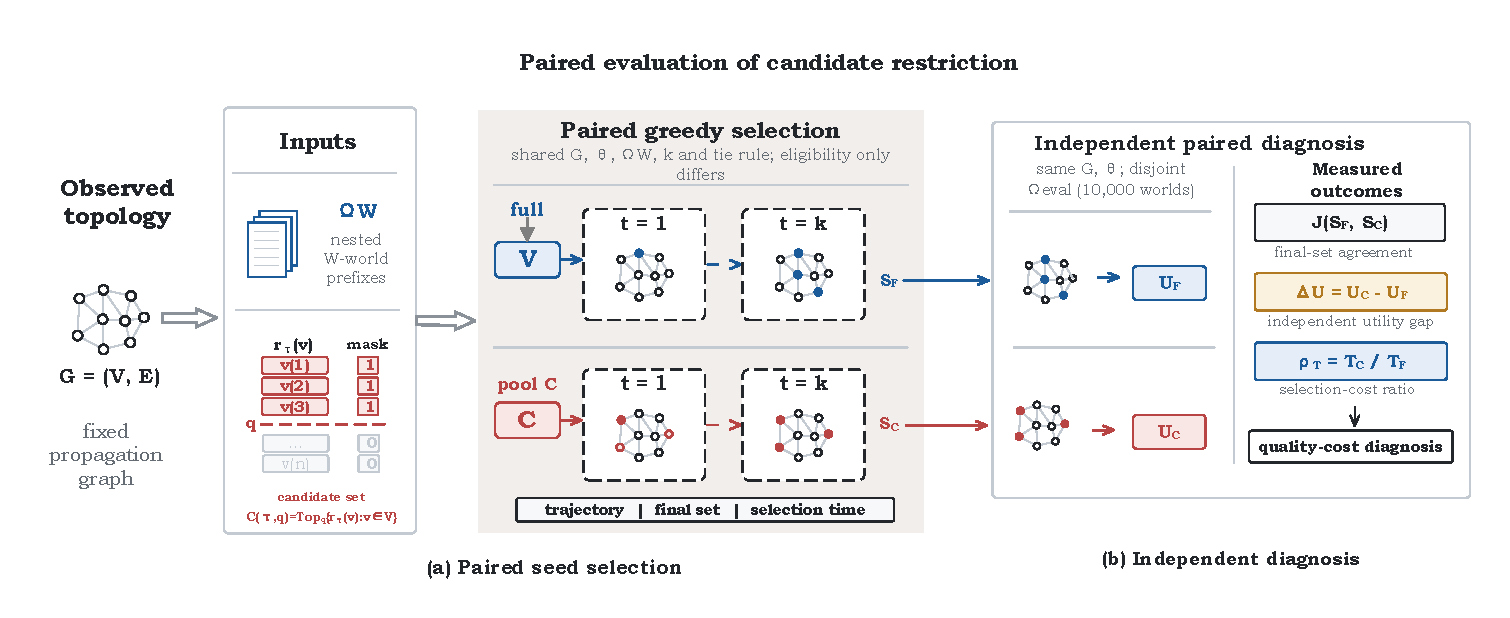
\includegraphics[width=\linewidth]{FigEvaluationMechanism.pdf}
\caption{Paired evaluation \DIFdelbeginFL \DIFdelFL{separates selection sampling, candidate ranking and independent utility assessment}\DIFdelendFL \DIFaddbeginFL \DIFaddFL{design}\DIFaddendFL . (a) \DIFdelbeginFL \DIFdelFL{Both arms select seeds using the same $W$ worlds. Ranking tolerance $\tau$ }\DIFdelendFL \DIFaddbeginFL \DIFaddFL{Full }\DIFaddendFL and \DIFdelbeginFL \DIFdelFL{cutoff $q$ define the }\DIFdelendFL restricted \DIFdelbeginFL \DIFdelFL{pool $C(\tau,q)$. Both arms }\DIFdelendFL \DIFaddbeginFL \DIFaddFL{greedy selection }\DIFaddendFL share the graph, \DIFdelbeginFL \DIFdelFL{world }\DIFdelendFL \DIFaddbeginFL \DIFaddFL{the propagation parameters $\theta$, the nested }\DIFaddendFL prefix \DIFaddbeginFL \DIFaddFL{of $W$ selection worlds}\DIFaddendFL , \DIFaddbeginFL \DIFaddFL{the }\DIFaddendFL seed budget \DIFaddbeginFL \DIFaddFL{$k$ }\DIFaddendFL and \DIFaddbeginFL \DIFaddFL{the }\DIFaddendFL tie rule. \DIFaddbeginFL \DIFaddFL{They differ only in the eligible set: the restricted method searches the pool $C(\tau,q)$ of the $q$ top-ranked vertices, with scores computed at tolerance $\tau$. }\DIFaddendFL (b) \DIFdelbeginFL \DIFdelFL{A separate, }\DIFdelendFL \DIFaddbeginFL \DIFaddFL{Both selected sets are evaluated on a }\DIFaddendFL shared family of \DIFdelbeginFL \DIFdelFL{$M=10,000$ evaluation }\DIFdelendFL \DIFaddbeginFL \DIFaddFL{$M=10{,}000$ }\DIFaddendFL worlds\DIFdelbeginFL \DIFdelFL{yields $\Delta U$}\DIFdelendFL , \DIFaddbeginFL \DIFaddFL{disjoint from the selection worlds. The outputs are the spread difference $\Delta U$ (}\DIFaddendFL restricted minus \DIFdelbeginFL \DIFdelFL{full-reference spread. Set agreement }\DIFdelendFL \DIFaddbeginFL \DIFaddFL{full), the final-set Jaccard similarity }\DIFaddendFL $J$ and \DIFdelbeginFL \DIFdelFL{selection-cost }\DIFdelendFL \DIFaddbeginFL \DIFaddFL{the selection-time }\DIFaddendFL ratio $\rho_T$\DIFdelbeginFL \DIFdelFL{complete the quality--cost comparison}\DIFdelendFL .}\label{fig:evaluation-mechanism}
\end{figure}

\section{Related work}
\paragraph{\DIFdelbegin \DIFdel{Objectives, sampling and computational efficiency}\DIFdelend \DIFaddbegin \DIFadd{Efficient greedy selection}\DIFaddend .} Kempe et al. \DIFdelbegin \DIFdel{establish monotonicity and submodularity of }\DIFdelend \DIFaddbegin \DIFadd{show that }\DIFaddend expected spread under the independent-cascade model \DIFdelbegin \DIFdel{, supporting greedy approximation }\DIFdelend \DIFaddbegin \DIFadd{is monotone and submodular, which gives greedy selection its approximation guarantee }\DIFaddend \cite{ref1}. CELF \DIFdelbegin \DIFdel{exploits submodularity to avoid unnecessary marginal reevaluations }\DIFdelend \DIFaddbegin \DIFadd{uses submodularity to skip re-evaluations of marginal gains that cannot change the current choice }\DIFaddend \cite{ref7}. StaticGreedy \DIFdelbegin \DIFdel{reuses fixed sampled realizations throughout selection, preserving a consistent sampled }\DIFdelend \DIFaddbegin \DIFadd{fixes one set of sampled realizations for the whole search, so that every candidate is scored on the same }\DIFaddend coverage objective \cite{ref8}\DIFdelbegin \DIFdel{. IMM develops }\DIFdelend \DIFaddbegin \DIFadd{, and IMM replaces forward simulation with }\DIFaddend a sampling-based solver \DIFdelbegin \DIFdel{with }\DIFdelend \DIFaddbegin \DIFadd{that carries }\DIFaddend approximation guarantees \cite{ref2}. These \DIFdelbegin \DIFdel{approaches address the computational difficulty of optimization under specified objectives. Their results motivate careful treatment of the sampled objective, but do not identify the utility consequence of excluding vertices through }\DIFdelend \DIFaddbegin \DIFadd{methods make a given objective cheaper to optimize. Candidate restriction instead shrinks the feasible set, and its effect on spread depends on which vertices }\DIFaddend a particular truncated ranking \DIFdelbegin \DIFdel{. Our comparison holds }\DIFdelend \DIFaddbegin \DIFadd{leaves out. In our experiments }\DIFaddend the simulator and \DIFdelbegin \DIFdel{greedy rule fixed while changing eligibility, the shared }\DIFdelend \DIFaddbegin \DIFadd{the greedy rule stay fixed, and only the eligible set, the }\DIFaddend selection budget or \DIFdelbegin \DIFdel{ranking tolerance}\DIFdelend \DIFaddbegin \DIFadd{the ranking tolerance changes}\DIFaddend .

\paragraph{Influence estimation and \DIFdelbegin \DIFdel{seed-selection strategies}\DIFdelend \DIFaddbegin \DIFadd{seed search}\DIFaddend .} Rui et al. estimate influence from multiple neighbourhood levels \cite{ref12}, \DIFdelbegin \DIFdel{while }\DIFdelend Fan et al. \DIFdelbegin \DIFdel{use }\DIFdelend \DIFaddbegin \DIFadd{search for seeds with a }\DIFaddend discrete Harris hawks \DIFdelbegin \DIFdel{optimization for seed selection \cite{ref13}. }\DIFdelend \DIFaddbegin \DIFadd{optimizer \cite{ref13}, and }\DIFaddend Ko et al.'s MONSTOR+ predicts spread on unseen graphs \cite{ref19}. \DIFdelbegin \DIFdel{These studies offer different ways to estimate influence or search for seed sets. Their algorithmic objectives differ from assessing a fixed ranking solely as a filter on seed eligibility. In the latter setting, greedy selection still operates }\DIFdelend \DIFaddbegin \DIFadd{Each of these methods supplies its own estimator or search procedure. We study a narrower role for a ranking: it decides only which vertices greedy search may select, while propagation and evaluation still run }\DIFaddend on the complete \DIFdelbegin \DIFdel{propagation graph, and candidate coverage becomes part of the comparison. We therefore distinguish a ranking 's role in defining the pool from the simulator's role in evaluating its selected seeds}\DIFdelend \DIFaddbegin \DIFadd{graph. In this role, the quality of a ranking appears as candidate coverage, that is, whether its pool contains the vertices that the full search would choose}\DIFaddend .

\paragraph{Evaluation \DIFdelbegin \DIFdel{settings and the remaining question}\DIFdelend \DIFaddbegin \DIFadd{of influence-maximization methods}\DIFaddend .} Li et al. survey \DIFdelbegin \DIFdel{influence-maximization methods }\DIFdelend \DIFaddbegin \DIFadd{the field }\DIFaddend \cite{ref9}, and Arora et al. \DIFdelbegin \DIFdel{examine their quality and computational cost in a benchmarking study }\DIFdelend \DIFaddbegin \DIFadd{benchmark the spread and running time of established methods }\DIFaddend \cite{ref16}. Yanchenko et al. review \DIFdelbegin \DIFdel{temporal-network formulations \cite{ref11}; }\DIFdelend \DIFaddbegin \DIFadd{formulations on temporal networks \cite{ref11}, and }\DIFaddend Aral and Dhillon study \DIFdelbegin \DIFdel{empirical influence }\DIFdelend \DIFaddbegin \DIFadd{influence maximization under empirically estimated influence }\DIFaddend models \cite{ref15}. Together, these \DIFdelbegin \DIFdel{research directions place algorithm comparisons within their diffusion models, network representations and evaluation settings. Our experiments use observed topologies with simulated diffusion. They assess sensitivity within that computational setting and do not estimate realized social influence.
}%DIFDELCMD < 

%DIFDELCMD < %%%
\DIFdel{For a truncated ranking, the comparison involves two computations. The ranking determines which vertices enter the search, and the sampled objective determines which eligible vertices become seeds. We vary these computations separately and measure their consequences }\DIFdelend \DIFaddbegin \DIFadd{studies tie any comparison of algorithms to a diffusion model, a network representation and an evaluation protocol. Our study concerns the protocol. When a cheaper search is compared with a sampled full-candidate reference, we ask how much of the observed gap comes from the restriction itself and how much from the selection budget and the ranking computation, and we measure each contribution }\DIFaddend on independent evaluation worlds.

\section{Methods}
We compare full and restricted greedy selection on the same propagation graph. \DIFdelbegin \DIFdel{The selection objective , evaluation metric and timing procedure are defined below. Network characteristics }\DIFdelend \DIFaddbegin \DIFadd{Section~\ref{sec:paired} defines the selection objective and the terms used throughout, Section~\ref{sec:coupling} the construction of selection and evaluation worlds, and Section~\ref{sec:cost} the cost measurement. Network statistics }\DIFaddend and parameter values \DIFdelbegin \DIFdel{appear }\DIFdelend \DIFaddbegin \DIFadd{are given }\DIFaddend in Section~\ref{sec:experimental-setup}.
\subsection{Paired \DIFaddbegin \DIFadd{greedy }\DIFaddend selection\DIFdelbegin \DIFdel{at controlled resolutions}\DIFdelend }\DIFaddbegin \label{sec:paired}
\DIFaddend Let $G=(V,E)$ be a directed propagation graph and $S$ a seed set of size $k$. Under the independent-cascade model, each newly activated vertex gets one opportunity to activate each inactive outgoing neighbour with probability $p$. Propagation stops after $h$ rounds. For a random world $\omega$, let $f_h(S;\omega)$ denote total activated vertices, including seeds. Greedy selection uses the sampled objective
\begin{equation}
\widehat\sigma_W(S)=\frac{1}{W}\sum_{w=1}^{W}f_h(S;\omega_w).
\end{equation}
\DIFdelbegin \DIFdel{At }\DIFdelend \DIFaddbegin \DIFadd{In }\DIFaddend each round, greedy selection \DIFdelbegin \DIFdel{enumerates }\DIFdelend \DIFaddbegin \DIFadd{evaluates }\DIFaddend every unselected eligible vertex \DIFdelbegin \DIFdel{and chooses the }\DIFdelend \DIFaddbegin \DIFadd{$v$ and adds the one with the }\DIFaddend largest integer total \DIFdelbegin \DIFdel{$W\widehat\sigma_W$. Ties resolve by lexicographic original node ID}\DIFdelend \DIFaddbegin \DIFadd{$W\widehat\sigma_W(S\cup\{v\})$. Comparing integer totals rather than floating-point means makes ties exact, and remaining ties are broken by the lexicographic order of original node IDs}\DIFaddend . Full selection uses $C=V$ \DIFdelbegin \DIFdel{; restricted selection uses $C\subseteq V$. All vertices remain in the propagation graph. A path identifies }\DIFdelend \DIFaddbegin \DIFadd{and restricted selection a pool $C\subset V$; in both cases propagation runs on the complete graph.
}

\DIFadd{We use the following terms throughout. A \emph{method} is a rule that defines the eligible set: full selection, or a restricted pool such as Degree-4k or PageRank-5\%. A \emph{replicate} is }\DIFaddend one computational repetition \DIFdelbegin \DIFdel{and its random-world families . A condition }\DIFdelend \DIFaddbegin \DIFadd{with its own families of selection and evaluation worlds, identified by a number (1101--1105 on the SNAP networks). A \emph{configuration} }\DIFaddend fixes the graph, \DIFdelbegin \DIFdel{path and experimental settings; an arm specifies a seed-eligibility rule within that condition. Full and restricted arms share $G$, the world prefix, }\DIFdelend \DIFaddbegin \DIFadd{the replicate, the selection budget $W$ and the world coupling; all methods in a configuration share the same worlds, seed budget }\DIFaddend $k$ and \DIFdelbegin \DIFdel{the }\DIFdelend tie rule. \DIFaddbegin \DIFadd{The \emph{full reference} is full selection in the same configuration, and every restricted method is compared with it.
}\DIFaddend 

In \DIFdelbegin \DIFdel{the budget sweeps, }\DIFdelend \DIFaddbegin \DIFadd{a budget sweep, the full reference and each restricted method are rerun at every }\DIFaddend $W$ \DIFdelbegin \DIFdel{governs seed selection for both the full-candidate reference and every restricted arm. Each arm selects its seeds anew at each $W$, using }\DIFdelend \DIFaddbegin \DIFadd{on }\DIFaddend the same nested \DIFdelbegin \DIFdel{world prefix . Candidate pools remain fixed}\DIFdelend \DIFaddbegin \DIFadd{prefix of selection worlds, while the candidate pool stays fixed. A change in their gap }\DIFaddend across $W$ \DIFdelbegin \DIFdel{within a given ranking setting; ranking }\DIFdelend \DIFaddbegin \DIFadd{can therefore come from either search. The ranking }\DIFaddend tolerance $\tau$ and \DIFaddbegin \DIFadd{the }\DIFaddend pool size $q$ are \DIFdelbegin \DIFdel{controlled separately . The resulting relative differences reflect changes in both selection procedures, rather than improvement of the reference alone.
}\DIFdelend \DIFaddbegin \DIFadd{varied separately from $W$.
}\DIFaddend 

Degree \DIFdelbegin \DIFdel{ranks distinct outgoing neighbours. PageRank uses }\DIFdelend \DIFaddbegin \DIFadd{is the number of distinct out-neighbours. PageRank is computed on }\DIFaddend the unweighted directed \DIFdelbegin \DIFdel{topology and }\DIFdelend \DIFaddbegin \DIFadd{graph with the }\DIFaddend NetworkX 3.5 defaults: damping \DIFdelbegin \DIFdel{.85}\DIFdelend \DIFaddbegin \DIFadd{0.85}\DIFaddend , uniform personalization and dangling-node \DIFdelbegin \DIFdel{treatment, tolerance $10^{-6}$ }\DIFdelend \DIFaddbegin \DIFadd{handling, tolerance $\tau=10^{-6}$ }\DIFaddend and at most 100 iterations \cite{networkxpr}. \DIFdelbegin \DIFdel{Its stopping criterion is successive-vector }\DIFdelend \DIFaddbegin \DIFadd{Iteration stops when the }\DIFaddend $L_1$ change \DIFaddbegin \DIFadd{between successive score vectors falls }\DIFaddend below $n\tau$, where $n=|V|$. \DIFdelbegin \DIFdel{Scores are sorted decreasingly with lexical ties . A top-$q$ pool contains }\DIFdelend \DIFaddbegin \DIFadd{Vertices are sorted by decreasing score, with ties broken lexicographically. A pool contains the top }\DIFaddend $q=\min(n,4k)$ \DIFdelbegin \DIFdel{or $q=\lceil .05n\rceil$ vertices . Historical weighted degree counts outgoing observed events where such counts exist. Three random pools are independently generated within each graph /path and }\DIFdelend \DIFaddbegin \DIFadd{vertices (4k pools) or the top $q=\lceil 0.05n\rceil$ vertices (5\% pools). Event-weighted degree counts messages sent on CollegeMsg and retained contact records incident to each vertex on the undirected contact networks. Each contact is represented by reciprocal arcs, giving each endpoint one outgoing record per retained contact (Weighted-4k and Weighted-5\%). As a baseline, three random pools of size $4k$ are drawn for each graph and replicate and held }\DIFaddend fixed across budgets and \DIFdelbegin \DIFdel{coupling controls}\DIFdelend \DIFaddbegin \DIFadd{couplings}\DIFaddend .

\subsection{World coupling and independent evaluation}\label{sec:coupling}
\DIFdelbegin \DIFdel{Primary selection worlds share draws }\DIFdelend \DIFaddbegin \DIFadd{The primary experiments use \emph{step coupling}, in which each random draw is }\DIFaddend indexed by world, propagation step, source and target. \DIFdelbegin \DIFdel{This coupling preserves the independent-cascade marginal law for each }\DIFdelend \DIFaddbegin \DIFadd{For any }\DIFaddend fixed seed set, \DIFdelbegin \DIFdel{but the realized finite-world objective can be nonmonotone. For example, initially activating }\DIFdelend \DIFaddbegin \DIFadd{this coupling reproduces the independent-cascade distribution of spread. The sampled objective, however, need not be monotone: seeding }\DIFaddend an intermediate vertex \DIFdelbegin \DIFdel{can move its outgoing attempt }\DIFdelend \DIFaddbegin \DIFadd{moves its activation attempts }\DIFaddend to an earlier step \DIFdelbegin \DIFdel{with a different sampled outcome. }\DIFdelend \DIFaddbegin \DIFadd{and hence to different draws, which can lower the realized spread (}\DIFaddend Online Resource 1 gives \DIFdelbegin \DIFdel{the explicit counterexample. A separate }\DIFdelend \DIFaddbegin \DIFadd{a counterexample). We retain the step coupling used in the earlier experiments for comparability and use }\DIFaddend fixed-edge \DIFdelbegin \DIFdel{control draws once per edge and world; its finite objective is coverage by vertices reachable }\DIFdelend \DIFaddbegin \DIFadd{sampling as a control. \emph{Fixed-edge coupling} draws each edge once per world. Its sampled objective counts the vertices reachable from $S$ }\DIFaddend within $h$ \DIFaddbegin \DIFadd{live }\DIFaddend edges and is monotone and submodular. \DIFdelbegin \DIFdel{Both implementations use exhaustive enumeration. }\DIFdelend \DIFaddbegin \DIFadd{At every round under both couplings, greedy search enumerates every eligible vertex that has not yet been selected. We use the same exhaustive search in both couplings. CELF can reuse marginal gains as upper bounds for the fixed-edge coverage objective; using that shortcut for the step-coupled objective would require a diminishing-returns guarantee. Each restricted method is compared with the full reference under its own coupling.
}\DIFaddend 

\DIFdelbegin \DIFdel{Selection-world identifiers }\DIFdelend \DIFaddbegin \DIFadd{Selection worlds }\DIFaddend form nested prefixes\DIFdelbegin \DIFdel{as }\DIFdelend \DIFaddbegin \DIFadd{: raising }\DIFaddend $W$ \DIFdelbegin \DIFdel{increases. In the external study and the 520-condition historical extension, evaluation uses $M=10,000$ }\DIFdelend \DIFaddbegin \DIFadd{appends worlds without redrawing the earlier ones. Evaluation uses $M=10{,}000$ }\DIFaddend worlds per graph\DIFdelbegin \DIFdel{/path/coupling, disjoint from selection and fixed across arms and budgets. Keys also separate graphs, paths and candidate-pool randomization.
Coupling schemes are compared within their own full references.
}\DIFdelend \DIFaddbegin \DIFadd{, replicate and coupling. These worlds are disjoint from the selection worlds and shared by all methods and budgets, both in the SNAP experiments and in the 520-configuration extension of the contact-graph study. Separate keys distinguish graphs, replicates and random-pool draws.
}\DIFaddend 

For restricted seeds $S_C$ and full-reference seeds $S_F$, define the paired evaluation difference on world $i$ as $d_i=f_h(S_C;\eta_i)-f_h(S_F;\eta_i)$. Both sets are selected at the same $W$; positive $d_i$ favors the restricted method. The utility gap in Fig.~\ref{fig:evaluation-mechanism} is
\begin{equation}
\widehat\Delta=\frac{1}{M}\sum_{i=1}^{M}d_i,
\qquad \operatorname{SE}_{\rm MC}=s(d_i)/\sqrt M.
\end{equation}
The interval $\widehat\Delta\pm1.96\operatorname{SE}_{\rm MC}$ \DIFdelbegin \DIFdel{describes conditional }\DIFdelend \DIFaddbegin \DIFadd{measures the }\DIFaddend Monte Carlo uncertainty \DIFdelbegin \DIFdel{for fixed selected sets. Across-path standard deviation describes variation across computational paths, including finite }\DIFdelend \DIFaddbegin \DIFadd{of the gap between two fixed seed sets. The standard deviation across replicates reflects how the selected sets themselves vary from one replicate to the next, together with the remaining }\DIFaddend evaluation noise. \DIFdelbegin \DIFdel{The three random-pool }\DIFdelend \DIFaddbegin \DIFadd{For the random pools, the three }\DIFaddend evaluation vectors are averaged within each \DIFdelbegin \DIFdel{path before either calculation}\DIFdelend \DIFaddbegin \DIFadd{replicate before either quantity is computed}\DIFaddend .

\DIFdelbegin \DIFdel{We report ordered-trajectory agreement, final-set agreement, Jaccard similarity and the first divergent round }\DIFdelend \DIFaddbegin \DIFadd{Agreement with the full reference is reported at three levels: an identical ordered seed sequence, an identical final set, and the Jaccard similarity of the final sets. We also record the first round at which the two sequences diverge}\DIFaddend . Incremental spread \DIFdelbegin \DIFdel{subtracts }\DIFdelend \DIFaddbegin \DIFadd{is total spread minus the }\DIFaddend $k$ \DIFdelbegin \DIFdel{from total spread ; percentage incremental loss }\DIFdelend \DIFaddbegin \DIFadd{seeds. The percentage loss of a restricted method }\DIFaddend is $-100\widehat\Delta/(\widehat\sigma_{\rm full}-k)$\DIFdelbegin \DIFdel{. Negative loss favors }\DIFdelend \DIFaddbegin \DIFadd{, where $\widehat\sigma_{\rm full}$ is the mean total spread of the full reference on the $M$ evaluation worlds of the same replicate; a positive loss means that }\DIFaddend the restricted set \DIFaddbegin \DIFadd{reaches fewer vertices. Losses are computed per replicate and then averaged}\DIFaddend .
\DIFdelbegin \DIFdel{All observed denominators are positive.
}\DIFdelend 

\DIFdelbegin \DIFdel{The frozen primary tests compare }\DIFdelend \DIFaddbegin \DIFadd{For each graph, we use pre-specified two-sided paired sign tests at $W=1280$, with Holm correction across the three primary comparisons: }\DIFaddend Degree-4k, PageRank-4k and the \DIFdelbegin \DIFdel{within-path random mean with full selectionat $W=1280$. Each comparison uses a two-sided exact sign test; Holm correction covers the three comparisons within each graph}\DIFdelend \DIFaddbegin \DIFadd{mean of the three random pools, each against full selection}\DIFaddend . \DIFaddbegin \DIFadd{The protocol fixed these comparisons before the primary results were inspected. }\DIFaddend Zero differences are excluded from the tests and reported separately. \DIFdelbegin \DIFdel{Coverage}\DIFdelend \DIFaddbegin \DIFadd{The analyses of coverage}\DIFaddend , coupling and \DIFdelbegin \DIFdel{transition analyses are descriptive; worlds and paths are not independent networksamples}\DIFdelend \DIFaddbegin \DIFadd{budget transitions are descriptive, since replicates measure computational variability on a fixed network}\DIFaddend .

\subsection{Implementation and cost measurement}\DIFdelbegin \DIFdel{The Numba implementation stores }\DIFdelend \DIFaddbegin \label{sec:cost}
\DIFadd{The implementation uses Numba and records, for each configuration and method, the }\DIFaddend candidate IDs, \DIFdelbegin \DIFdel{selected sequences, integer round totals and }\DIFdelend \DIFaddbegin \DIFadd{the selected sequence, the integer totals of every round and the }\DIFaddend per-world evaluation values. \DIFdelbegin \DIFdel{Reproduction }\DIFdelend \DIFaddbegin \DIFadd{Online Resource 1 describes the reproduction }\DIFaddend and verification procedures\DIFdelbegin \DIFdel{are provided in Online Resource 1.}\footnote{\DIFdel{OpenAI Codex assisted with basic code development and manuscript drafting.}}
%DIFAUXCMD
\addtocounter{footnote}{-1}%DIFAUXCMD
\DIFdelend \DIFaddbegin \DIFadd{.
}\DIFaddend 

Selection time \DIFdelbegin \DIFdel{includes }\DIFdelend \DIFaddbegin \DIFadd{covers }\DIFaddend greedy search and \DIFdelbegin \DIFdel{lexical candidate sorting , but excludes }\DIFdelend \DIFaddbegin \DIFadd{the lexicographic sorting of candidates; }\DIFaddend graph preparation, world generation and evaluation \DIFdelbegin \DIFdel{. We also }\DIFdelend \DIFaddbegin \DIFadd{are timed separately. To }\DIFaddend estimate the cost of a \DIFdelbegin \DIFdel{warm-process run that includes independent evaluation. Separately measured }\DIFdelend \DIFaddbegin \DIFadd{complete run in a warm process, we add the separately measured costs of }\DIFaddend parsing, graph construction and one method's ranking \DIFdelbegin \DIFdel{/pool generation are added }\DIFdelend \DIFaddbegin \DIFadd{and pool construction (median of five repeats) }\DIFaddend to the recorded costs of \DIFdelbegin \DIFdel{selection-world preparation, seed selection , evaluation-world preparation and evaluation . Setup uses the median of five repeats. These assembled estimates exclude }\DIFdelend \DIFaddbegin \DIFadd{preparing selection worlds, selecting seeds, preparing evaluation worlds and evaluating. This assembled cost excludes }\DIFaddend imports, just-in-time compilation, downloads and output writing.

\DIFdelbegin \DIFdel{Five randomized repeats at path }\DIFdelend \DIFaddbegin \DIFadd{Timing variability is assessed with five repeats in randomized method order on replicate }\DIFaddend 1101 \DIFdelbegin \DIFdel{and }\DIFdelend \DIFaddbegin \DIFadd{at }\DIFaddend $W=320$\DIFdelbegin \DIFdel{assess timing variability. Cost comparisons use }\DIFdelend \DIFaddbegin \DIFadd{. All cost comparisons are made against }\DIFaddend this implementation's exhaustive full-candidate \DIFdelbegin \DIFdel{reference. Results at the tighter PageRank toleranceare used only for quality sensitivity; the timing comparison uses default tolerance }\DIFdelend \DIFaddbegin \DIFadd{search and use the default PageRank tolerance; the tighter tolerance enters only the quality analysis}\DIFaddend .

\DIFaddbegin \paragraph{\DIFadd{Use of AI tools.}} \DIFadd{OpenAI Codex assisted with basic code development and manuscript drafting. The authors take responsibility for the final manuscript.
}

\DIFaddend \section{Experimental setup}\label{sec:experimental-setup}
\DIFaddbegin \DIFadd{We study three SNAP networks under simulated independent-cascade diffusion with $k=5$, $p=0.01$ and $h=3$, and use an earlier contact-graph study from this project as a point of comparison.
}

\DIFaddend \paragraph{Inputs and outputs.} Each run takes \DIFdelbegin \DIFdel{the processed graph $G$, }\DIFdelend \DIFaddbegin \DIFadd{a processed graph with }\DIFaddend its arc directions, \DIFaddbegin \DIFadd{the diffusion parameters }\DIFaddend $k$, $p$ \DIFdelbegin \DIFdel{, }\DIFdelend \DIFaddbegin \DIFadd{and }\DIFaddend $h$, \DIFdelbegin \DIFdel{the shared }\DIFdelend \DIFaddbegin \DIFadd{a }\DIFaddend selection budget $W$ and a candidate rule. \DIFdelbegin \DIFdel{Ranking }\DIFdelend \DIFaddbegin \DIFadd{The ranking }\DIFaddend tolerance $\tau$ and \DIFaddbegin \DIFadd{the }\DIFaddend cutoff $q$ determine the restricted pool\DIFdelbegin \DIFdel{$C$; they leave }\DIFdelend \DIFaddbegin \DIFadd{, while }\DIFaddend the propagation graph \DIFaddbegin \DIFadd{stays }\DIFaddend intact. Selection returns an ordered sequence of $k$ seeds and its \DIFdelbegin \DIFdel{final set, together with }\DIFdelend selection time. \DIFdelbegin \DIFdel{Independent evaluation takes that set and }\DIFdelend \DIFaddbegin \DIFadd{Evaluation takes the final set and the }\DIFaddend $M$ \DIFdelbegin \DIFdel{held-out worlds , returning }\DIFdelend \DIFaddbegin \DIFadd{evaluation worlds of the replicate, and returns }\DIFaddend total spread, incremental spread and \DIFdelbegin \DIFdel{paired differences from the same-budget full reference }\DIFdelend \DIFaddbegin \DIFadd{the paired difference from the full reference at the same $W$}\DIFaddend . Tables~\ref{tab:primary} and~\ref{tab:case} \DIFdelbegin \DIFdel{connect these outputs to }\DIFdelend \DIFaddbegin \DIFadd{show these outputs together with }\DIFaddend candidate counts and original node IDs.

\subsection{Networks and preprocessing}
We selected three \DIFdelbegin \DIFdel{larger SNAP topologies before inspecting }\DIFdelend \DIFaddbegin \DIFadd{SNAP networks of different types before inspecting any }\DIFaddend seed sets or \DIFdelbegin \DIFdel{utilities }\DIFdelend \DIFaddbegin \DIFadd{spreads }\DIFaddend \cite{snap}: CollegeMsg \DIFdelbegin \DIFdel{communication}\DIFdelend \DIFaddbegin \DIFadd{(communication)}\DIFaddend , ca-GrQc \DIFdelbegin \DIFdel{collaboration }\DIFdelend \DIFaddbegin \DIFadd{(collaboration) }\DIFaddend and wiki-Vote \DIFdelbegin \DIFdel{voting}\DIFdelend \DIFaddbegin \DIFadd{(voting)}\DIFaddend . Table~\ref{tab:data} \DIFdelbegin \DIFdel{reports the }\DIFdelend \DIFaddbegin \DIFadd{lists their }\DIFaddend processed sizes and candidate coverage\DIFdelbegin \DIFdel{. All retained components are included}\DIFdelend \DIFaddbegin \DIFadd{; all weak components are retained}\DIFaddend .
\begin{table}[htbp]
\caption{Processed SNAP networks. Arcs are directed propagation arcs. The 4k fraction is the share of vertices in a 20-vertex pool; the 5\% pool contains $\lceil 0.05n\rceil$ vertices.}\label{tab:data}
\begin{tabular}{lrrrr}
\toprule
Graph & Nodes & Arcs & 4k fraction & 5\% pool \\
\midrule
CollegeMsg & 1,438 & 13,397 & 1.391\% & 72 \\
ca-GrQc & 5,241 & 28,968 & 0.382\% & 263 \\
wiki-Vote & 7,115 & 103,689 & 0.281\% & 356 \\
\bottomrule
\end{tabular}
\end{table}

CollegeMsg records timestamped \DIFdelbegin \DIFdel{sender-to-receiver messages \cite{college}. We sort its 58, 911 }\DIFdelend \DIFaddbegin \DIFadd{messages from sender to receiver \cite{college}. Following the history-window convention of the contact-graph study, we retain the earliest 65\% of }\DIFaddend distinct timestamps, \DIFdelbegin \DIFdel{retain the first $\lfloor .65\times58,911\rfloor=38,292$ complete groups,and include events through Unix timestamp }\DIFdelend \DIFaddbegin \DIFadd{$\lfloor 0.65\times58{,}911\rfloor=38{,}292$ of 58,911, which covers events up to Unix time }\DIFaddend 1085640224. \DIFdelbegin \DIFdel{Removing }\DIFdelend \DIFaddbegin \DIFadd{After removing }\DIFaddend self-messages\DIFdelbegin \DIFdel{leaves }\DIFdelend \DIFaddbegin \DIFadd{, we use the }\DIFaddend 38,939 \DIFdelbegin \DIFdel{events. Repeated sender--receiver pairs contribute to historical outgoing-message counts but }\DIFdelend \DIFaddbegin \DIFadd{retained events both to construct the directed graph and to rank vertices by outgoing message count. Repeated messages between the same pair }\DIFaddend form a single propagation arc \DIFdelbegin \DIFdel{. Propagation uses }\DIFdelend \DIFaddbegin \DIFadd{but each count toward the sender's message count, and propagation uses the }\DIFaddend uniform $p$ \DIFdelbegin \DIFdel{, independently of the }\DIFdelend \DIFaddbegin \DIFadd{regardless of }\DIFaddend message count.

ca-GrQc \DIFdelbegin \DIFdel{links coauthors \cite{grqc}; we }\DIFdelend \DIFaddbegin \DIFadd{connects coauthors \cite{grqc}. We }\DIFaddend remove self-loops, \DIFdelbegin \DIFdel{deduplicate pairs and create reciprocal arcs . Vertices are collected after loop removal, excluding the self-loop-only vertex }\DIFdelend \DIFaddbegin \DIFadd{merge duplicate pairs and add arcs in both directions. Vertex }\DIFaddend 12295 \DIFdelbegin \DIFdel{and giving }\DIFdelend \DIFaddbegin \DIFadd{appears only in a self-loop and is dropped, which leaves }\DIFaddend 5,241 \DIFdelbegin \DIFdel{rather than the source page's }\DIFdelend \DIFaddbegin \DIFadd{vertices instead of the }\DIFaddend 5,242 \DIFdelbegin \DIFdel{vertices. }\DIFdelend \DIFaddbegin \DIFadd{listed by SNAP. In }\DIFaddend wiki-Vote\DIFdelbegin \DIFdel{arcs run }\DIFdelend \DIFaddbegin \DIFadd{, arcs point }\DIFaddend from voter to votee \cite{signed,links}; \DIFaddbegin \DIFadd{we remove }\DIFaddend self-loops and duplicate arcs \DIFdelbegin \DIFdel{are removed without reversing the remaining arcs. Outgoing diffusion on these arcs is a simulation assumption. The }\DIFdelend \DIFaddbegin \DIFadd{and keep the original direction, so that influence is simulated as flowing from voters to the users they vote for. Because the }\DIFaddend two static datasets \DIFdelbegin \DIFdel{provide topology-only inputs; historical-weighted ranking requires event counts. We retain all weak components: }\DIFdelend \DIFaddbegin \DIFadd{carry no event counts, event-weighted pools are used only on CollegeMsg. The processed graphs have }\DIFaddend 2 \DIFdelbegin \DIFdel{in CollegeMsg}\DIFdelend \DIFaddbegin \DIFadd{(CollegeMsg)}\DIFaddend , 354 \DIFdelbegin \DIFdel{in }\DIFdelend \DIFaddbegin \DIFadd{(}\DIFaddend ca-GrQc\DIFaddbegin \DIFadd{) }\DIFaddend and 24 \DIFdelbegin \DIFdel{in }\DIFdelend \DIFaddbegin \DIFadd{(}\DIFaddend wiki-Vote\DIFaddbegin \DIFadd{) weak components}\DIFaddend . Original IDs are stored as strings and sorted lexicographically \DIFdelbegin \DIFdel{for graph indexing, ranking ties and greedy ties. Raw-file and processed-graph hashes are supplied }\DIFdelend \DIFaddbegin \DIFadd{to index vertices and to break ties in ranking and in greedy selection. Hashes of the raw and processed files are listed }\DIFaddend in the data manifest.

\DIFdelbegin \DIFdel{Historical context comes from four contact-derived }\DIFdelend \DIFaddbegin \DIFadd{The earlier stage of this project used four contact }\DIFaddend graphs with 75--402 vertices, \DIFdelbegin \DIFdel{constructed }\DIFdelend \DIFaddbegin \DIFadd{derived }\DIFaddend from workplace, conference and rural Kenya data \cite{ref3,ref4,ref5,ref6}. \DIFdelbegin \DIFdel{We distinguish four evidence layers: the initial 42-condition study; a 520-condition historical extension; the external matrix below; and its post-hoc PageRank precision control. The extension uses ten paths per contact graphand }\DIFdelend \DIFaddbegin \DIFadd{It began with 42 configurations and was later extended to 520 configurations with ten replicates per graph. The extension }\DIFaddend adds a budget scan up to $W=5120$, four local changes to $(p,h)$, fixed-edge sampling, a larger seed budget \DIFaddbegin \DIFadd{of $k=20$}\DIFaddend , and two fixed 2,000-node synthetic \DIFdelbegin \DIFdel{instances \cite{ref17,ref18}. The parameter controls reuse the default budget-scan conditions}\DIFdelend \DIFaddbegin \DIFadd{graphs \cite{ref17,ref18}; the parameter variations reuse the configurations of the default budget scan}\DIFaddend . Online Resource 1 reports the \DIFdelbegin \DIFdel{complete coverage and descriptive results separately}\DIFdelend \DIFaddbegin \DIFadd{contact-graph results in full}\DIFaddend .

\subsection{Primary \DIFdelbegin \DIFdel{matrix }\DIFdelend \DIFaddbegin \DIFadd{design }\DIFaddend and \DIFdelbegin \DIFdel{numerical sensitivity control}\DIFdelend \DIFaddbegin \DIFadd{ranking-precision analysis}\DIFaddend }
Table~\ref{tab:settings} \DIFdelbegin \DIFdel{specifies the external design . Here, conditions vary graph, path, selection budget and coupling; the remaining propagation settings are fixed. Three }\DIFdelend \DIFaddbegin \DIFadd{summarizes the design on the SNAP networks. The primary experiments cross three }\DIFaddend graphs, five \DIFdelbegin \DIFdel{paths }\DIFdelend \DIFaddbegin \DIFadd{replicates }\DIFaddend and three selection budgets\DIFdelbegin \DIFdel{define }\DIFdelend \DIFaddbegin \DIFadd{, $W\in\{80,320,1280\}$, which gives }\DIFaddend 45 \DIFdelbegin \DIFdel{primary conditions. Nine }\DIFdelend \DIFaddbegin \DIFadd{configurations under step coupling. Nine further configurations use }\DIFaddend fixed-edge \DIFdelbegin \DIFdel{conditions provide a matched coupling control. Every condition includes }\DIFdelend \DIFaddbegin \DIFadd{coupling at $W=320$ on replicates 1101--1103. Every configuration runs }\DIFaddend full selection, Degree-4k, PageRank-4k, Degree-5\%, PageRank-5\% and three \DIFdelbegin \DIFdel{random-4k pools; CollegeMsg also includes }\DIFdelend \DIFaddbegin \DIFadd{random 4k pools, and CollegeMsg adds }\DIFaddend Weighted-4k and Weighted-5\%\DIFdelbegin \DIFdel{pools based on outgoing message counts. This gives }\DIFdelend \DIFaddbegin \DIFadd{. Over the }\DIFaddend 18 \DIFdelbegin \DIFdel{conditions }\DIFdelend \DIFaddbegin \DIFadd{configurations }\DIFaddend per graph, \DIFdelbegin \DIFdel{with 10 arms for CollegeMsg and 8 for each static graph: $18(10+8+8)=468$ arms.
All 54 conditions were completed and retained.
}\DIFdelend \DIFaddbegin \DIFadd{this amounts to $18\times(10+8+8)=468$ method runs.
}\DIFaddend 

\begin{table}[htbp]
\caption{Experiment settings on the SNAP networks.}\label{tab:settings}
\begin{tabularx}{\linewidth}{lX}
\toprule
Quantity & Setting \\
\midrule
Diffusion & Independent cascade; uniform $p=0.01$; horizon $h=3$; $k=5$ seeds \\
Primary selection & Step coupling; $W\in\{80,320,1280\}$; replicates 1101--1105 \\
Evaluation & $M=10{,}000$ worlds per graph, replicate and coupling, shared across methods and budgets \\
Pool sizes & $4k=20$ or $\lceil0.05n\rceil$; three random pools of size 20 per replicate \\
Fixed-edge control & $W=320$; replicates 1101--1103 \\
Default PageRank & Damping 0.85; $\tau=10^{-6}$; at most 100 iterations \\
Strict PageRank (post-hoc) & $\tau=10^{-12}$; at most 1,000 iterations; pool unchanged at $10^{-14}$ \\
Repeated timing & Five repeats per method in randomized order; replicate 1101, $W=320$ \\
\bottomrule
\end{tabularx}
\end{table}

The \DIFdelbegin \DIFdel{external budget sweep spans 80 to 1280 selection worlds. At each budget both arms select five seeds, with $p=.01$ and $h=3$. The historical contact-graph sweep extends to $W=5120$.
}%DIFDELCMD < 

%DIFDELCMD < %%%
\DIFdel{The post-hoc PageRank control uses }\DIFdelend \DIFaddbegin \DIFadd{ranking-precision analysis was added after the primary results were available. On }\DIFaddend the original five \DIFdelbegin \DIFdel{paths. At each $W$}\DIFdelend \DIFaddbegin \DIFadd{replicates}\DIFaddend , it recomputes \DIFdelbegin \DIFdel{the restricted seeds with tolerance $10^{-12}$ }\DIFdelend \DIFaddbegin \DIFadd{PageRank with $\tau=10^{-12}$ }\DIFaddend and at most 1,000 iterations, \DIFdelbegin \DIFdel{then compares them }\DIFdelend \DIFaddbegin \DIFadd{reruns the restricted search at each $W$, and compares the result }\DIFaddend with the original full reference on the same evaluation worlds. \DIFdelbegin \DIFdel{The resulting candidate pools have identical membership at $10^{-12}$ and $10^{-14}$}\DIFdelend \DIFaddbegin \DIFadd{Recomputing at $\tau=10^{-14}$ leaves the pool membership unchanged}\DIFaddend . Online Resource 1 describes the two stages of this \DIFdelbegin \DIFdel{control}\DIFdelend \DIFaddbegin \DIFadd{analysis}\DIFaddend .

\subsection{Randomization, execution and reproducibility}
\DIFdelbegin \DIFdel{World identifiers }\DIFdelend \DIFaddbegin \DIFadd{All random draws are derived from hash keys that }\DIFaddend separate graphs, \DIFdelbegin \DIFdel{paths and selection/}\DIFdelend \DIFaddbegin \DIFadd{replicates, and the selection and }\DIFaddend evaluation families. \DIFdelbegin \DIFdel{Increasing }\DIFdelend \DIFaddbegin \DIFadd{Raising }\DIFaddend $W$ appends selection worlds without resampling the prefix\DIFdelbegin \DIFdel{; the }\DIFdelend \DIFaddbegin \DIFadd{, and we verify that }\DIFaddend selection and evaluation identifiers \DIFdelbegin \DIFdel{are checked for }\DIFdelend \DIFaddbegin \DIFadd{never }\DIFaddend overlap. Random \DIFdelbegin \DIFdel{candidate }\DIFdelend pools use a separate \DIFdelbegin \DIFdel{randomization }\DIFdelend key and remain fixed across budgets and \DIFdelbegin \DIFdel{coupling controls}\DIFdelend \DIFaddbegin \DIFadd{couplings}\DIFaddend . Online Resource 1 \DIFdelbegin \DIFdel{, }\DIFdelend \DIFaddbegin \DIFadd{(}\DIFaddend ``Executable reproduction procedure''\DIFdelbegin \DIFdel{, specifies the exact hash keys, }\DIFdelend \DIFaddbegin \DIFadd{) gives the exact keys, the }\DIFaddend identifier construction and \DIFdelbegin \DIFdel{hash-to-draw mapping }\DIFdelend \DIFaddbegin \DIFadd{the mapping from hashes to draws}\DIFaddend .

Experiments \DIFdelbegin \DIFdel{use one }\DIFdelend \DIFaddbegin \DIFadd{run as a single }\DIFaddend serial worker on Windows with Python 3.13.0, NumPy 2.3.3, NetworkX 3.5, SciPy 1.16.1 and Numba 0.68.0\DIFdelbegin \DIFdel{. BLAS /OpenMP threads are constrained to one . JIT warm-up precedes timed conditions; randomized arm order reduces systematic order effects. The recorded host has }\DIFdelend \DIFaddbegin \DIFadd{, with BLAS and OpenMP limited to one thread, on a host with }\DIFaddend 20 physical \DIFdelbegin \DIFdel{CPU cores and approximately }\DIFdelend \DIFaddbegin \DIFadd{cores and about }\DIFaddend 32 GiB \DIFdelbegin \DIFdel{RAM.
}\DIFdelend \DIFaddbegin \DIFadd{of RAM. Just-in-time compilation is warmed up before any timed configuration, and methods run in randomized order to avoid systematic order effects.
}\DIFaddend 

\section{Results}
\subsection{\DIFdelbegin \DIFdel{An apparent }\DIFdelend \DIFaddbegin \DIFadd{Post-hoc sensitivity of the }\DIFaddend budget \DIFdelbegin \DIFdel{reversal depends on ranking precision}\DIFdelend \DIFaddbegin \DIFadd{comparison to PageRank tolerance}\DIFaddend }
On ca-GrQc, \DIFdelbegin \DIFdel{does }\DIFdelend the direction of the PageRank-4k comparison depend\DIFaddbegin \DIFadd{s}\DIFaddend  on the tolerance \DIFdelbegin \DIFdel{used to rank candidates? At }\DIFdelend \DIFaddbegin \DIFadd{at which PageRank is computed (Fig.~\ref{fig:precision-budget}, Table~\ref{tab:precision-output}). At the }\DIFaddend default tolerance, \DIFdelbegin \DIFdel{mean relative incremental spread was 5.61\% above the same-budget full reference }\DIFdelend \DIFaddbegin \DIFadd{PageRank-4k exceeds the full reference by a mean 5.6\% of incremental spread }\DIFaddend at $W=80$, then \DIFdelbegin \DIFdel{2.53\% and 5.07}\DIFdelend \DIFaddbegin \DIFadd{falls 2.5\% and 5.1}\DIFaddend \% below it at $W=320$ and \DIFdelbegin \DIFdel{1280. At tighter toleranceit was above }\DIFdelend \DIFaddbegin \DIFadd{1,280. At the strict tolerance, it exceeds }\DIFaddend the reference at all three budgets, by \DIFdelbegin \DIFdel{11.25\%, 2.96\% and 0.54\%, respectively (Fig.
~\ref{fig:precision-budget}).
}\DIFdelend \DIFaddbegin \DIFadd{11.3\%, 3.0\% and 0.5\%. This analysis is post-hoc, and the gaps involved are small: at most 0.49 nodes in magnitude, against a full-reference incremental spread of 4.9 nodes at $W=1280$, with across-replicate standard deviations of 0.08--0.27 nodes.
}\DIFaddend 

\DIFdelbegin \DIFdel{Tightening tolerance removed }\DIFdelend \DIFaddbegin \DIFadd{Two vertices change at the pool boundary. Tightening the tolerance removes }\DIFaddend vertices 1488 and 19865 from the \DIFdelbegin \DIFdel{20-node pool and admitted }\DIFdelend \DIFaddbegin \DIFadd{20-vertex pool and admits }\DIFaddend 17655 and \DIFdelbegin \DIFdel{6610. At each budget, this exchange changed }\DIFdelend \DIFaddbegin \DIFadd{6610, which changes }\DIFaddend the final seed set on all five \DIFdelbegin \DIFdel{paths (Table~\ref{tab:precision-output}). At $W=1280$, the strict-minus-full spread difference averaged $+0.02608$ nodes, ranging from $-0.0408$ to $+0.1789$ across paths (SD 0.09155). Holding the strict poolfixed and increasing }\DIFdelend \DIFaddbegin \DIFadd{replicates at every budget. The selection budget still matters within the strict pool: raising }\DIFaddend $W$ \DIFdelbegin \DIFdel{changed }\DIFdelend \DIFaddbegin \DIFadd{changes }\DIFaddend the selected set on \DIFdelbegin \DIFdel{3/5 paths }\DIFdelend \DIFaddbegin \DIFadd{three of five replicates }\DIFaddend from 80 to 320 \DIFdelbegin \DIFdel{and 2/5 }\DIFdelend \DIFaddbegin \DIFadd{worlds and on two }\DIFaddend from 320 to \DIFdelbegin \DIFdel{1280.
}\DIFdelend \DIFaddbegin \DIFadd{1,280. At $W=1280$ the strict gap averages $+0.026$ nodes and ranges from $-0.041$ to $+0.179$ across replicates, so it lies on both sides of zero.
}\DIFaddend 

\DIFdelbegin \DIFdel{CollegeMsg's default- and tighter-tolerance }\DIFdelend \DIFaddbegin \DIFadd{On the two directed networks, the PageRank-4k losses persist at the tighter tolerance. On CollegeMsg, the two tolerances yield identical }\DIFaddend pools, seeds and evaluations\DIFdelbegin \DIFdel{are identical at every budget, retaining losses of 9.33\%, 8.52\% and 9.01\% }\DIFdelend \DIFaddbegin \DIFadd{, with losses of 9.3\%, 8.5\% and 9.0\% at the three budgets}\DIFaddend . On wiki-Vote \DIFdelbegin \DIFdel{, }\DIFdelend one candidate changes, but \DIFdelbegin \DIFdel{losses at the tighter tolerance remain 74.05\% , 74.05\% and 73.96\%}\DIFdelend \DIFaddbegin \DIFadd{the loss at the strict tolerance remains about 74\% at every budget}\DIFaddend .

\begin{table}[htbp]
\caption{PageRank-4k on ca-GrQc at the default ($\tau=10^{-6}$) and strict ($\tau=10^{-12}$) tolerance. Gaps are restricted minus full-reference spread at the same $W$, in nodes, averaged over five replicates, with the standard deviation across replicates in parentheses. Changed sets counts the replicates on which the two tolerances select different final sets.}\label{tab:precision-output}
\centering\begin{tabular}{rrrr}\toprule
$W$ & Default gap (SD) & Strict gap (SD) & Changed sets \\ \midrule
80 & +0.23606 (0.27402) & +0.48570 (0.24999) & 5/5 \\
320 & -0.12632 (0.18077) & +0.13804 (0.17387) & 5/5 \\
1280 & -0.25082 (0.07636) & +0.02608 (0.09155) & 5/5 \\
\bottomrule\end{tabular}
\end{table}

\begin{figure}[t]
\centering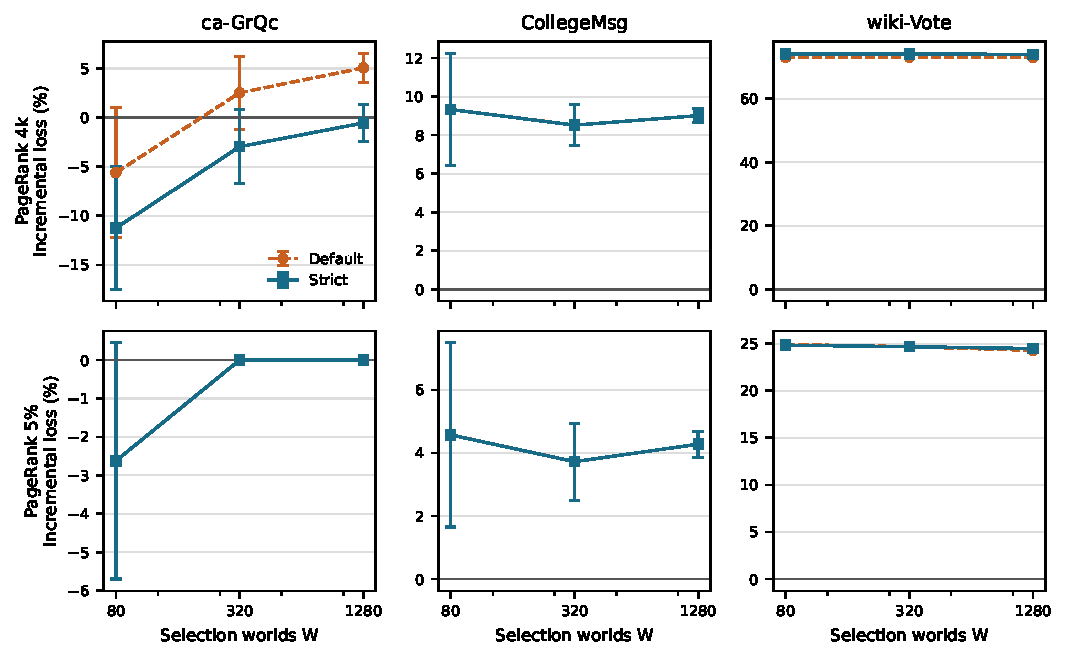
\includegraphics[width=\linewidth]{Fig4.pdf}
\caption{\DIFdelbeginFL \DIFdelFL{Selection budget and ranking precision have distinct effects on candidate-restriction quality. At each $W$, restricted methods are compared with }\DIFdelendFL \DIFaddbeginFL \DIFaddFL{Incremental-spread loss of PageRank pools relative to }\DIFaddendFL the full reference \DIFdelbeginFL \DIFdelFL{selected }\DIFdelendFL at \DIFdelbeginFL \DIFdelFL{that }\DIFdelendFL \DIFaddbeginFL \DIFaddFL{the }\DIFaddendFL same $W$\DIFaddbeginFL \DIFaddFL{, at the default ($\tau=10^{-6}$) and strict ($\tau=10^{-12}$) tolerance. Top row: 4k pools}\DIFaddendFL ; \DIFdelbeginFL \DIFdelFL{evaluation uses fixed independent worlds}\DIFdelendFL \DIFaddbeginFL \DIFaddFL{bottom row: 5\% pools}\DIFaddendFL . Points are \DIFdelbeginFL \DIFdelFL{mean incremental losses }\DIFdelendFL \DIFaddbeginFL \DIFaddFL{means }\DIFaddendFL over five \DIFdelbeginFL \DIFdelFL{paired paths; }\DIFdelendFL \DIFaddbeginFL \DIFaddFL{replicates and }\DIFaddendFL bars are \DIFdelbeginFL \DIFdelFL{path }\DIFdelendFL standard deviations \DIFdelbeginFL \DIFdelFL{. The plotted labels Default and Strict denote tolerances $10^{-6}$ and $10^{-12}$}\DIFdelendFL \DIFaddbeginFL \DIFaddFL{across replicates}\DIFaddendFL ; \DIFdelbeginFL \DIFdelFL{candidate membership is unchanged between $10^{-12}$ and $10^{-14}$. Negative }\DIFdelendFL \DIFaddbeginFL \DIFaddFL{a positive }\DIFaddendFL loss \DIFdelbeginFL \DIFdelFL{favors }\DIFdelendFL \DIFaddbeginFL \DIFaddFL{means that }\DIFaddendFL the restricted set \DIFaddbeginFL \DIFaddFL{reaches fewer vertices}\DIFaddendFL . \DIFdelbeginFL \DIFdelFL{The }\DIFdelendFL \DIFaddbeginFL \DIFaddFL{On }\DIFaddendFL ca-GrQc\DIFaddbeginFL \DIFaddFL{, the }\DIFaddendFL default \DIFdelbeginFL \DIFdelFL{reversal disappears with }\DIFdelendFL \DIFaddbeginFL \DIFaddFL{PageRank-4k loss changes sign across budgets, whereas }\DIFaddendFL the \DIFdelbeginFL \DIFdelFL{tighter PageRank tolerance}\DIFdelendFL \DIFaddbeginFL \DIFaddFL{strict-tolerance loss stays below zero. On CollegeMsg and wiki-Vote}\DIFaddendFL , \DIFdelbeginFL \DIFdelFL{while }\DIFdelendFL the \DIFdelbeginFL \DIFdelFL{directed-network }\DIFdelendFL losses persist \DIFaddbeginFL \DIFaddFL{at both tolerances}\DIFaddendFL .\DIFdelbeginFL \DIFdelFL{This is a post-hoc paired sensitivity analysis.}\DIFdelendFL }\label{fig:precision-budget}
\end{figure}

\subsection{\DIFdelbegin \DIFdel{Changing }\DIFdelend \DIFaddbegin \DIFadd{A change in }\DIFaddend the reference set \DIFdelbegin \DIFdel{does }\DIFdelend \DIFaddbegin \DIFadd{need }\DIFaddend not \DIFdelbegin \DIFdel{determine the spread }\DIFdelend change \DIFdelbegin %DIFDELCMD < \MBLOCKRIGHTBRACE
%DIFDELCMD < %%%
\DIFdel{For the full reference , we compared the }\DIFdelend \DIFaddbegin \DIFadd{its }\DIFaddend spread\DIFdelbegin \DIFdel{of the seeds selected at $W=1280$ with that of the seeds selected at $W=320$ on each path }\DIFdelend \DIFaddbegin }
\DIFadd{The full reference often changes as $W$ grows, but the resulting change in spread is small and can take either sign }\DIFaddend (Fig.~\ref{fig:transitions}). \DIFdelbegin \DIFdel{All }\DIFdelend \DIFaddbegin \DIFadd{Between $W=320$ and 1,280, all }\DIFaddend five ca-GrQc \DIFdelbegin \DIFdel{sets changed. Their mean spread changewas $+0.12720$ nodes, with individual differences from $-0.0266$ to $+0.2411$}\DIFdelend \DIFaddbegin \DIFadd{reference sets change, and their spread changes by a mean $+0.127$ nodes, ranging from $-0.027$ to $+0.241$}\DIFaddend . On CollegeMsg one set \DIFdelbegin \DIFdel{changed, and spread increased by 0.05336 nodeson average across all five paths}\DIFdelend \DIFaddbegin \DIFadd{changes, which raises the five-replicate mean spread by 0.053 nodes}\DIFaddend . On wiki-Vote some selection orders \DIFdelbegin \DIFdel{changed, but every final set was identical across budgets and every paired spread difference was zero. }%DIFDELCMD < 

%DIFDELCMD < %%%
\DIFdelend \DIFaddbegin \DIFadd{change but no final set does; because spread depends only on the set, every paired difference is exactly zero. }\DIFaddend Of the six changed sets, four have \DIFdelbegin \DIFdel{positive pointwise }\DIFdelend 95\% \DIFdelbegin \DIFdel{conditional }\DIFdelend Monte Carlo intervals \DIFdelbegin \DIFdel{; two}\DIFdelend \DIFaddbegin \DIFadd{above zero, and the intervals of the other two, both on }\DIFaddend ca-GrQc\DIFdelbegin \DIFdel{intervals }\DIFdelend \DIFaddbegin \DIFadd{, }\DIFaddend include zero.
\DIFdelbegin \DIFdel{The nine unchanged sets have identical evaluation vectors.
}\DIFdelend 

\DIFdelbegin \DIFdel{In the historical step-coupled comparison from $W=1280$ to 5120}\DIFdelend \DIFaddbegin \DIFadd{The contact-graph study shows the same pattern at larger budgets. Under step coupling}\DIFaddend , 16 \DIFdelbegin \DIFdel{/}\DIFdelend \DIFaddbegin \DIFadd{of }\DIFaddend 40 \DIFdelbegin \DIFdel{sets changed while the mean high-minus-low budget spread change was 0.01111 }\DIFdelend \DIFaddbegin \DIFadd{reference sets change between $W=1280$ and 5,120, while spread changes by a mean $+0.011$ }\DIFaddend nodes (range \DIFdelbegin \DIFdel{$-0.0383$ to $+0.1180$). Historical }\DIFdelend \DIFaddbegin \DIFadd{$-0.038$ to $+0.118$). Under }\DIFaddend fixed-edge \DIFdelbegin \DIFdel{references also change: from $W=320$ to 1280}\DIFdelend \DIFaddbegin \DIFadd{coupling}\DIFaddend , 29 \DIFdelbegin \DIFdel{/}\DIFdelend \DIFaddbegin \DIFadd{of }\DIFaddend 40 sets \DIFdelbegin \DIFdel{changed,with mean high-minus-low budget spread change 0.061845 }\DIFdelend \DIFaddbegin \DIFadd{change between $W=320$ and 1,280, with a mean change of $+0.062$ }\DIFaddend nodes (range \DIFdelbegin \DIFdel{$-0.0110$ to $+0.2572$}\DIFdelend \DIFaddbegin \DIFadd{$-0.011$ to $+0.257$}\DIFaddend ). Each transition \DIFdelbegin \DIFdel{uses a shared evaluation family }\DIFdelend \DIFaddbegin \DIFadd{is evaluated on a shared family of worlds }\DIFaddend within its own coupling\DIFdelbegin \DIFdel{. Because the two budget intervals differ, their mean changes do not estimate a coupling effect}\DIFdelend \DIFaddbegin \DIFadd{, and the two span different budget ranges}\DIFaddend .
\begin{figure}[t]
\centering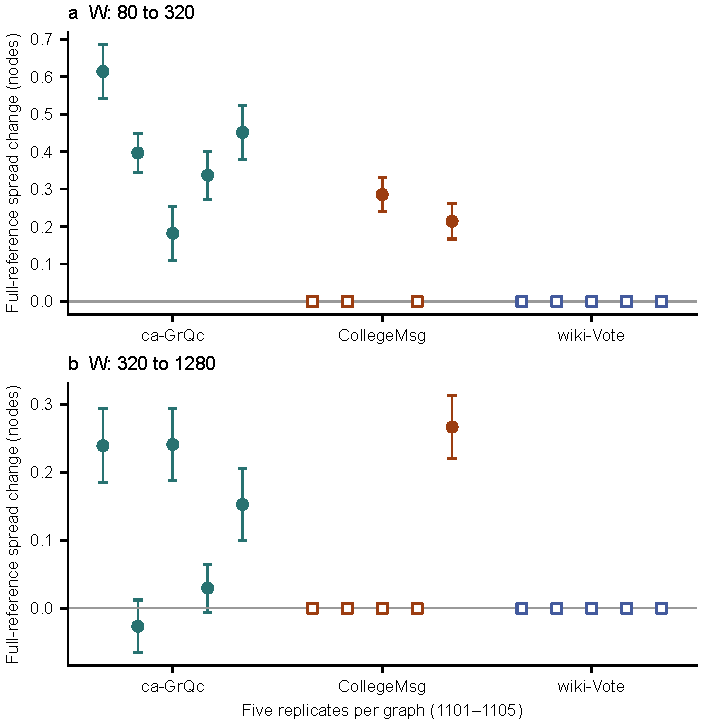
\includegraphics[width=\linewidth]{Fig2.pdf}
\caption{\DIFdelbeginFL \DIFdelFL{Reference-set changes and independent spread changes, defined as higher-budget minus lower-budget }\DIFdelendFL \DIFaddbeginFL \DIFaddFL{Change in }\DIFaddendFL full-reference spread \DIFdelbeginFL \DIFdelFL{. Filled circles denote changed final sets}\DIFdelendFL \DIFaddbeginFL \DIFaddFL{between two selection budgets (higher minus lower $W$) for each replicate on the SNAP networks: (a) $W=80$ to 320}\DIFaddendFL ; \DIFdelbeginFL \DIFdelFL{hollow squares denote unchanged sets. Paths }\DIFdelendFL \DIFaddbeginFL \DIFaddFL{(b) $W=320$ to 1,280. Replicates }\DIFaddendFL 1101--1105 run from left to right within each graph. \DIFaddbeginFL \DIFaddFL{Filled circles mark replicates whose final set changed, and hollow squares mark unchanged sets. }\DIFaddendFL Bars are unadjusted 95\% \DIFdelbeginFL \DIFdelFL{conditional }\DIFdelendFL Monte Carlo intervals from 10,000 paired \DIFaddbeginFL \DIFaddFL{evaluation }\DIFaddendFL worlds. \DIFdelbeginFL \DIFdelFL{Panel-specific vertical }\DIFdelendFL \DIFaddbeginFL \DIFaddFL{Vertical }\DIFaddendFL scales \DIFdelbeginFL \DIFdelFL{reveal small changes; the intervals condition on selected sets and do not describe variation across networks}\DIFdelendFL \DIFaddbeginFL \DIFaddFL{differ between panels}\DIFaddendFL .}\label{fig:transitions}
\end{figure}

\subsection{\DIFdelbegin \DIFdel{Ranking agreement depends on coverage and network context}\DIFdelend \DIFaddbegin \DIFadd{Degree pools reproduce the reference, PageRank pools do not}\DIFaddend }
At $W=1280$, Degree-4k reproduces every \DIFdelbegin \DIFdel{full-candidate reference trajectory across the three external graphs using }\DIFdelend \DIFaddbegin \DIFadd{full-reference seed sequence on all three SNAP networks while searching }\DIFaddend only 20 candidates (Table~\ref{tab:primary}). Default PageRank-4k \DIFdelbegin \DIFdel{matches none and incurs mean incremental losses of }\DIFdelend \DIFaddbegin \DIFadd{reproduces none and loses a mean }\DIFaddend \GrqcPRLoss{}\%, \CollegePRLoss{}\% and \WikiPRLoss{}\% \DIFaddbegin \DIFadd{of incremental spread }\DIFaddend on ca-GrQc, CollegeMsg and wiki-Vote. The \DIFdelbegin \DIFdel{historical extension showed much broader PageRank agreement : }\DIFdelend \DIFaddbegin \DIFadd{contact-graph study found near-complete agreement for both rankings: PageRank-4k reproduced }\DIFaddend 40 \DIFdelbegin \DIFdel{/}\DIFdelend \DIFaddbegin \DIFadd{of }\DIFaddend 40 \DIFdelbegin \DIFdel{trajectories }\DIFdelend \DIFaddbegin \DIFadd{sequences }\DIFaddend at $W=5120$ \DIFdelbegin \DIFdel{, compared with }\DIFdelend \DIFaddbegin \DIFadd{and Degree-4k }\DIFaddend 39 \DIFdelbegin \DIFdel{/40 for degree. The external results therefore limit transfer of the contact-graph ranking result.
}\DIFdelend \DIFaddbegin \DIFadd{of 40. The earlier PageRank agreement thus varies across the networks and budgets examined here.
}

\DIFaddend \begin{table}[htbp]
\caption{Results on the SNAP networks at $W=1280$, averaged over five replicates. PR denotes PageRank at the default tolerance. Incremental spread excludes the $k=5$ seeds; the gap is restricted minus full-reference spread, in nodes; agreement counts replicates with an identical ordered seed sequence.}\label{tab:primary}
\centering\begin{tabular}{lrrrr}\toprule
Graph / method & Candidates & Incremental & Gap & Agreement \\ \midrule
\multicolumn{5}{l}{\textit{ca-GrQc}} \\
Full & 5241 & 4.934 & --- & --- \\
Degree-4k & 20 & 4.934 & +0.00000 & 5/5 \\
PR-4k & 20 & 4.683 & -0.25082 & 0/5 \\
PR-5\% & 263 & 4.934 & +0.00000 & 5/5 \\
\addlinespace
\multicolumn{5}{l}{\textit{CollegeMsg}} \\
Full & 1438 & 10.072 & --- & --- \\
Degree-4k & 20 & 10.072 & +0.00000 & 5/5 \\
PR-4k & 20 & 9.164 & -0.90780 & 0/5 \\
PR-5\% & 72 & 9.641 & -0.43094 & 0/5 \\
\addlinespace
\multicolumn{5}{l}{\textit{wiki-Vote}} \\
Full & 7115 & 55.736 & --- & --- \\
Degree-4k & 20 & 55.736 & +0.00000 & 5/5 \\
PR-4k & 20 & 15.043 & -40.69334 & 0/5 \\
PR-5\% & 356 & 42.206 & -13.53012 & 0/5 \\
\bottomrule\end{tabular}
\end{table}

\DIFdelbegin \DIFdel{On }\DIFdelend \DIFaddbegin \DIFadd{In the pre-specified tests at $W=1280$, the PageRank-4k difference and the random-pool mean difference from full selection are negative on every replicate of every graph, which gives an unadjusted sign-test $p=0.0625$ and a Holm-adjusted $p=0.1875$. With five replicates, 0.0625 is the smallest attainable two-sided $p$-value, so these consistent losses cannot reach conventional significance. The Degree-4k differences are exactly zero. Online Resource 1 reports the paired effect sizes and the complete test results.
}

\DIFadd{Table~\ref{tab:case} illustrates the contrast on }\DIFaddend wiki-Vote \DIFdelbegin \DIFdel{path 1101, the 20-node Degree pool returned }\DIFdelend \DIFaddbegin \DIFadd{replicate 1101. The 20-vertex degree pool returns }\DIFaddend the same five seeds, in the same order, as the full search over 7,115 vertices\DIFdelbegin \DIFdel{(Table~\ref{tab:case}). Their }\DIFdelend \DIFaddbegin \DIFadd{, and reaches a }\DIFaddend mean total spread \DIFdelbegin \DIFdel{was 60.8455 nodes. With the same pool size, default PageRank selected }\DIFdelend \DIFaddbegin \DIFadd{of 60.8 nodes. Default PageRank-4k selects }\DIFaddend five different seeds and \DIFdelbegin \DIFdel{reached 19.9366 nodes. Expanding }\DIFdelend \DIFaddbegin \DIFadd{reaches 19.9 nodes; enlarging }\DIFaddend its pool to 356 vertices \DIFdelbegin \DIFdel{raised spread to 47.2095.
Table~\ref{tab:primary} gives the corresponding five-path comparison for each network.
}\DIFdelend \DIFaddbegin \DIFadd{raises this to 47.2 nodes.
}

\DIFaddend \begin{table}[htbp]
\caption{Selected seeds on wiki-Vote, replicate 1101 ($k=5$, $p=0.01$, $h=3$, $W=1280$, $M=10{,}000$, step coupling; 7,115 vertices and 103,689 arcs). PR uses the default tolerance. Arrows give the selection order; total spread includes the seeds and is estimated on the evaluation worlds.}\label{tab:case}
\begin{tabularx}{\linewidth}{lXr}\toprule
Method & Selected seed sequence & Total spread \\ \midrule
Full & $2565\to 766\to 11\to 457\to 2688$ & 60.8455 \\
Degree-4k & $2565\to 766\to 11\to 457\to 2688$ & 60.8455 \\
PR-4k & $3352\to 2237\to 2328\to 2654\to 1297$ & 19.9366 \\
PR-5\% & $2565\to 1166\to 1549\to 1374\to 5524$ & 47.2095 \\
\bottomrule\end{tabularx}
\end{table}

\DIFdelbegin \DIFdel{For the primary comparisons at the highest tested external budget, every default PageRank-4k and within-path random-4k mean difference from full selection is negative, giving unadjusted sign-test $p=.0625$ and within-graph Holm $p=.1875$. Degree-4k differences from full selection are exactly zero. Five paths limit the minimum two-sided sign-test value to .0625. The paired effect sizes, sensitivity controls and complete test results are reported in Online Resource 1.
}%DIFDELCMD < 

%DIFDELCMD < %%%
\DIFdel{Increasing the default PageRank pool to }\DIFdelend \DIFaddbegin \DIFadd{Larger pools reduce the PageRank loss, but by different amounts on different networks. With the }\DIFaddend 5\% \DIFaddbegin \DIFadd{pool, PageRank }\DIFaddend reproduces all five ca-GrQc references at $W=1280$ and \DIFdelbegin \DIFdel{reduces }\DIFdelend \DIFaddbegin \DIFadd{cuts the }\DIFaddend CollegeMsg loss from \CollegePRLoss{}\% to \CollegePRfiveLoss{}\%. On wiki-Vote \DIFdelbegin \DIFdel{, }\DIFdelend \DIFaddbegin \DIFadd{the }\DIFaddend loss falls from \WikiPRLoss{}\% to \WikiPRfiveLoss{}\%, \DIFdelbegin \DIFdel{remaining above one fifth of full-reference }\DIFdelend \DIFaddbegin \DIFadd{which is still more than a fifth of the reference's }\DIFaddend incremental spread. \DIFdelbegin \DIFdel{At the same budget, historical-weighted CollegeMsg}\DIFdelend \DIFaddbegin \DIFadd{On CollegeMsg, event-weighted }\DIFaddend pools move from a \DIFdelbegin \DIFdel{negative mean difference of $-0.25224$ }\DIFdelend \DIFaddbegin \DIFadd{mean gap of $-0.25$ }\DIFaddend nodes at 4k to exact \DIFdelbegin \DIFdel{reference reproduction }\DIFdelend \DIFaddbegin \DIFadd{reproduction of the reference }\DIFaddend at 5\%.
\DIFdelbegin \DIFdel{Coverage helps in these comparisons, but its effect differs across networks.
}\DIFdelend 

On wiki-Vote, the \DIFdelbegin \DIFdel{default }\DIFdelend \DIFaddbegin \DIFadd{two 20-vertex pools draw on different kinds of vertices. The }\DIFaddend PageRank top 20 have \DIFaddbegin \DIFadd{a }\DIFaddend mean in-degree \DIFdelbegin \DIFdel{249.75 and }\DIFdelend \DIFaddbegin \DIFadd{of 250 and a mean }\DIFaddend out-degree \DIFdelbegin \DIFdel{56.2; }\DIFdelend \DIFaddbegin \DIFadd{of 56, whereas }\DIFaddend the degree top 20 have \DIFdelbegin \DIFdel{mean in-degree 70.3 and out-degree 489.25. }\DIFdelend \DIFaddbegin \DIFadd{70 and 489. }\DIFaddend The PageRank-4k pool contains none of the five full-reference seeds on any \DIFaddbegin \DIFadd{replicate at }\DIFaddend $W=1280$\DIFdelbegin \DIFdel{path, and its }\DIFdelend \DIFaddbegin \DIFadd{, and the }\DIFaddend 5\% pool contains only one. \DIFdelbegin \DIFdel{The }\DIFdelend \DIFaddbegin \DIFadd{Online Resource 1 gives the }\DIFaddend seed-level illustration and \DIFaddbegin \DIFadd{the }\DIFaddend complete coverage comparisons\DIFdelbegin \DIFdel{appear in Online Resource 1.
}\DIFdelend \DIFaddbegin \DIFadd{.
}\DIFaddend 

\subsection{\DIFdelbegin \DIFdel{Reference-preserving savings under specified timing scopes}\DIFdelend \DIFaddbegin \DIFadd{Degree-4k preserves the reference at a fraction of the selection cost}\DIFaddend }
\DIFaddbegin \DIFadd{At $W=1280$, }\DIFaddend Degree-4k reduces \DIFdelbegin \DIFdel{measured }\DIFdelend selection time by \DIFdelbegin \DIFdel{98.40}\DIFdelend \DIFaddbegin \DIFadd{98.4}\DIFaddend --99\DIFdelbegin \DIFdel{.67}\DIFdelend \DIFaddbegin \DIFadd{.7}\DIFaddend \% relative to \DIFdelbegin \DIFdel{this implementation's }\DIFdelend \DIFaddbegin \DIFadd{exhaustive }\DIFaddend full-candidate \DIFdelbegin \DIFdel{reference at $W=1280$, while reproducing all its trajectories }\DIFdelend \DIFaddbegin \DIFadd{search while reproducing every reference sequence }\DIFaddend (Table~\ref{tab:cost}). \DIFdelbegin \DIFdel{Including }\DIFdelend \DIFaddbegin \DIFadd{When graph }\DIFaddend setup, both world families and independent evaluation \DIFdelbegin \DIFdel{gives assembled cost savings of }\DIFdelend \DIFaddbegin \DIFadd{are included, the saving is }\DIFaddend \CollegeDegreeSaving{}--\WikiDegreeSaving{}\%\DIFdelbegin \DIFdel{.
}\DIFdelend \DIFaddbegin \DIFadd{, because both methods incur graph and world preparation costs. This estimate includes each method's own ranking or pool-construction cost and its measured evaluation time.
}

\DIFaddend \begin{table}[htbp]
\caption{Selection cost of Degree-4k at $W=1280$, averaged over five replicates. Full and Degree give the measured selection time. The last column gives the saving in an assembled warm-process cost that adds graph setup, preparation of selection and evaluation worlds, and independent evaluation (Section~\ref{sec:cost}).}\label{tab:cost}
\begin{tabular}{lrrrr}
\toprule
Graph & Full (s) & Degree (s) & \shortstack{Selection\\saving (\%)} & \shortstack{Saving including\\evaluation (\%)} \\
\midrule
ca-GrQc & 23.53 & 0.109 & 99.54 & 92.77 \\
CollegeMsg & 5.89 & 0.094 & 98.40 & 86.59 \\
wiki-Vote & 158.94 & 0.520 & 99.67 & 96.26 \\
\bottomrule
\end{tabular}
\end{table}

\DIFaddbegin \DIFadd{We also report the fraction of replicates meeting each of six pre-specified loss thresholds (0\%, 1\%, 2.5\%, 5\%, 10\% and 20\%), with loss expressed relative to the full reference's incremental spread within each replicate. }\DIFaddend At $W=1280$, Degree-4k meets the \DIFdelbegin \DIFdel{zero point-estimate loss threshold relative to full selection on every path}\DIFdelend \DIFaddbegin \DIFadd{0\% threshold on every replicate}\DIFaddend . Default PageRank-4k meets \DIFaddbegin \DIFadd{the }\DIFaddend 10\% \DIFaddbegin \DIFadd{threshold }\DIFaddend on ca-GrQc and CollegeMsg \DIFdelbegin \DIFdel{, but fails }\DIFdelend \DIFaddbegin \DIFadd{but misses }\DIFaddend 20\% on every wiki-Vote \DIFdelbegin \DIFdel{path. None of the }\DIFdelend \DIFaddbegin \DIFadd{replicate, and no }\DIFaddend random-pool \DIFdelbegin \DIFdel{path means }\DIFdelend \DIFaddbegin \DIFadd{mean }\DIFaddend meets 20\%. Online Resource 1 \DIFdelbegin \DIFdel{reports all six frozen thresholds (0, 1, 2.5, 5, 10 and 20\%) and their cost estimates; these are descriptive criteria rather than application-validated tolerances}\DIFdelend \DIFaddbegin \DIFadd{lists the fractions for all thresholds and the corresponding costs}\DIFaddend .

\subsection{\DIFdelbegin \DIFdel{Parameter and }\DIFdelend \DIFaddbegin \DIFadd{Results under fixed-edge }\DIFaddend coupling \DIFdelbegin \DIFdel{controls delimit the findings}\DIFdelend \DIFaddbegin \DIFadd{and other parameters}\DIFaddend }
\DIFdelbegin %DIFDELCMD < 

%DIFDELCMD < %%%
\DIFdel{In the external }\DIFdelend \DIFaddbegin \DIFadd{The PageRank losses persist under }\DIFaddend fixed-edge \DIFdelbegin \DIFdel{control at }\DIFdelend \DIFaddbegin \DIFadd{coupling. At }\DIFaddend $W=320$, default PageRank-4k \DIFdelbegin \DIFdel{minus }\DIFdelend \DIFaddbegin \DIFadd{trails }\DIFaddend the fixed-edge full reference \DIFdelbegin \DIFdel{has mean spread differences of $-0.16240$, $-0.93417$ and $-40.57597$ }\DIFdelend \DIFaddbegin \DIFadd{by a mean 0.16, 0.93 and 40.6 }\DIFaddend nodes on ca-GrQc, CollegeMsg and wiki-Vote. Degree-4k reproduces \DIFaddbegin \DIFadd{one of the three reference sequences on ca-GrQc and all three on CollegeMsg and wiki-Vote. Online Resource }\DIFaddend 1 \DIFdelbegin \DIFdel{/3, 3/3 and 3/3 corresponding trajectories. The PageRank losses persist under this control , while some reference-agreement outcomes change. Complete control paths and repeated timings are supplied in Online Resource 1.
}\DIFdelend \DIFaddbegin \DIFadd{gives the complete control results and the repeated timings.
}\DIFaddend 

\DIFdelbegin \DIFdel{Across the }\DIFdelend \DIFaddbegin \DIFadd{In the contact-graph study, both rankings reproduce most full-reference sequences in the }\DIFaddend 160 \DIFdelbegin \DIFdel{historical nondefault parameter conditions }\DIFdelend \DIFaddbegin \DIFadd{configurations with non-default parameters }\DIFaddend at $W=320$\DIFdelbegin \DIFdel{, }\DIFdelend \DIFaddbegin \DIFadd{: 117 for }\DIFaddend Degree-4k and \DIFdelbegin \DIFdel{PageRank-4k reproduce 117 and }\DIFdelend 132 \DIFdelbegin \DIFdel{full-reference trajectories, respectively. Weighted-4k minus full selectionhas }\DIFdelend \DIFaddbegin \DIFadd{for PageRank-4k. Event-weighted pools mostly fall short of full selection, with }\DIFaddend 117 negative and 43 positive paired \DIFdelbegin \DIFdel{spread differences. }%DIFDELCMD < 

%DIFDELCMD < %%%
\DIFdel{Under historical }\DIFdelend \DIFaddbegin \DIFadd{differences. Under }\DIFaddend fixed-edge \DIFdelbegin \DIFdel{sampling }\DIFdelend \DIFaddbegin \DIFadd{coupling }\DIFaddend at $W=1280$, Degree-4k and PageRank-4k \DIFdelbegin \DIFdel{match }\DIFdelend \DIFaddbegin \DIFadd{reproduce }\DIFaddend 38 \DIFdelbegin \DIFdel{/40 }\DIFdelend and 40 \DIFdelbegin \DIFdel{/40 trajectories of the fixed-edge full reference , while }\DIFdelend \DIFaddbegin \DIFadd{of 40 reference sequences, whereas }\DIFaddend Weighted-4k \DIFdelbegin \DIFdel{matches 5/40.
}\DIFdelend \DIFaddbegin \DIFadd{reproduces 5.
}\DIFaddend \FloatBarrier

\section{Discussion}
\subsection{Why the ca-GrQc comparison changes sign}
\DIFdelbegin \DIFdel{At default PageRank tolerance, a budget sweep }\DIFdelend \DIFaddbegin \DIFadd{The reversal }\DIFaddend on ca-GrQc \DIFdelbegin \DIFdel{would rank the restricted method above the full reference at the lowest budgetand below it at the highest. Two candidate substitutions were enough to change that judgment. At }\DIFdelend \DIFaddbegin \DIFadd{comes from the candidate pool, not from the selection budget. At a }\DIFaddend fixed $W$, the \DIFaddbegin \DIFadd{two tolerance settings share the }\DIFaddend full reference, \DIFaddbegin \DIFadd{the }\DIFaddend sampled objective and \DIFdelbegin \DIFdel{evaluation worlds were common to both tolerance settings. The sign reversal therefore depended on which vertices were eligible. Increasing $W$ still changed seeds within the tighter pool, }\DIFdelend \DIFaddbegin \DIFadd{the evaluation worlds, and differ only in which vertices are eligible. Exchanging two of the 20 candidates is therefore enough to turn a budget sweep in which the restricted method appears to fall behind the reference into one in which it never does. The budget still has an effect of its own: within the strict pool, raising $W$ changes the selected seeds, }\DIFaddend and at the highest budget \DIFdelbegin \DIFdel{its spread differences lay on both sides of zero. }\DIFdelend \DIFaddbegin \DIFadd{the gap spans zero. A sweep over $W$ thus mixes two processes, the convergence of each search and the composition of the pool, and when the gaps amount to a fraction of a node, the second can decide the outcome.
}\DIFaddend 

StaticGreedy \DIFdelbegin \DIFdel{fixes sampled realizations during }\DIFdelend \DIFaddbegin \DIFadd{controls sampling variation by fixing the sampled realizations throughout }\DIFaddend the search \cite{ref8}\DIFdelbegin \DIFdel{. In our comparisons the same sampling control applies to both arms, but ranking and truncationprecede the search }\DIFdelend \DIFaddbegin \DIFadd{, and our paired design applies the same control to both searches. Ranking and truncation, however, act before the search begins and lie outside this control. Reporting which candidate IDs enter or leave the pool when the tolerance is tightened identifies the changes in eligibility}\DIFaddend .
\DIFdelbegin \DIFdel{Reporting the candidate IDs at the cutoff makes this earlier source of variation visible.
}\DIFdelend 

\subsection{\DIFdelbegin \DIFdel{When a different sequence changes spread}\DIFdelend \DIFaddbegin \DIFadd{Seed sequences and seed sets}\DIFaddend }
\DIFdelbegin \DIFdel{Seed order records the decisions made by greedy search. The diffusion model instead takes }\DIFdelend \DIFaddbegin \DIFadd{Agreement statistics based on seed sequences can overstate how much a change matters. Greedy search produces an ordered sequence, but the diffusion model takes only }\DIFaddend the final set as \DIFdelbegin \DIFdel{its input. On wiki-Vote, a change in order therefore }\DIFdelend \DIFaddbegin \DIFadd{input, so on wiki-Vote a reordered sequence }\DIFaddend left every evaluation count unchanged\DIFdelbegin \DIFdel{when the two budgets returned the same set. A change in membership admits a different outcome}\DIFdelend \DIFaddbegin \DIFadd{. When the membership does change, its effect on spread has to be measured}\DIFaddend : on ca-GrQc\DIFaddbegin \DIFadd{, }\DIFaddend the higher-budget \DIFaddbegin \DIFadd{reference }\DIFaddend sets reached more \DIFdelbegin \DIFdel{nodes on some paths }\DIFdelend \DIFaddbegin \DIFadd{vertices on some replicates }\DIFaddend and fewer on others. \DIFdelbegin \DIFdel{The relevant quantity for seeding }\DIFdelend \DIFaddbegin \DIFadd{For seeding decisions the relevant quantity }\DIFaddend is the paired spread difference\DIFdelbegin \DIFdel{on each path}\DIFdelend \DIFaddbegin \DIFadd{, and set agreement serves mainly to diagnose where that difference comes from}\DIFaddend .

\subsection{Candidate coverage and the cost of exclusion}
\DIFaddbegin \DIFadd{Increasing the PageRank pool size recovers part of the spread lost on wiki-Vote. }\DIFaddend On wiki-Vote, the \DIFdelbegin \DIFdel{default PageRank top 20 }\DIFdelend \DIFaddbegin \DIFadd{20-vertex PageRank pool }\DIFaddend excluded all five reference seeds\DIFdelbegin \DIFdel{. Among the top 356 candidates, one reference seed became eligible. Although the expanded pool could still reproduce at most onereference seed, its five-path }\DIFdelend \DIFaddbegin \DIFadd{, and the 356-vertex pool admitted only one. The larger pool nonetheless raised the five-replicate }\DIFaddend mean total spread \DIFdelbegin \DIFdel{rose from 20.04268 to 47.20590 }\DIFdelend \DIFaddbegin \DIFadd{from 20.0 to 47.2 }\DIFaddend nodes, against \DIFdelbegin \DIFdel{60.73602 }\DIFdelend \DIFaddbegin \DIFadd{60.7 }\DIFaddend for the full reference. \DIFaddbegin \DIFadd{Thus, at least four of the five seeds in each expanded-pool result differ from the corresponding reference seeds.
}\DIFaddend 

The two \DIFdelbegin \DIFdel{20-node pools differ in how they sample the directed graph. The PageRank candidates }\DIFdelend \DIFaddbegin \DIFadd{20-vertex pools favour opposite directions of the graph. PageRank promotes vertices that }\DIFaddend receive many votes, whereas \DIFdelbegin \DIFdel{the degree candidates have manydistinct outgoing neighbours. Since the simulator propagates from voter to votee, the observed loss is consistent with this directional difference }\DIFdelend \DIFaddbegin \DIFadd{degree promotes vertices that cast many}\DIFaddend . \DIFaddbegin \DIFadd{Diffusion follows voter-to-votee arcs, so a vertex with more distinct out-neighbours has more opportunities for first-round activation. This directional difference is consistent with the observed spread gap. }\DIFaddend Reversing the propagation direction on the same topology would \DIFdelbegin \DIFdel{directly test that interpretation }\DIFdelend \DIFaddbegin \DIFadd{test this interpretation directly}\DIFaddend .

\DIFaddbegin \DIFadd{Benchmarks such as that of }\DIFaddend Arora et al. \DIFdelbegin \DIFdel{compare the }\DIFdelend \DIFaddbegin \DIFadd{report }\DIFaddend spread and running time \DIFdelbegin \DIFdel{of influence-maximization methods \cite{ref16}. Here the timing comparison has a specific interpretation: }\DIFdelend \DIFaddbegin \DIFadd{side by side \cite{ref16}. Our results add that the same computational budget can buy very different quality depending on which ranking defines the pool. }\DIFaddend Degree-4k \DIFdelbegin \DIFdel{eliminated }\DIFdelend \DIFaddbegin \DIFadd{removes }\DIFaddend most candidate evaluations while \DIFdelbegin \DIFdel{retaining the reference sequence }\DIFdelend \DIFaddbegin \DIFadd{reproducing the reference }\DIFaddend on all 15 \DIFdelbegin \DIFdel{highest-budget paths. For default PageRank-4k on wiki-Vote, restricting the search to the same number of candidates incurred a 73.01\% mean incremental-spread loss.
Table~\ref{tab:cost} separates time spent selecting seeds from costs that also include preparation and evaluation.
}\DIFdelend \DIFaddbegin \DIFadd{graph--replicate pairs at $W=1280$, whereas a PageRank pool of the same size on wiki-Vote loses nearly three quarters of the incremental spread.
}\DIFaddend 

\subsection{Scope \DIFdelbegin \DIFdel{of the comparisons}\DIFdelend \DIFaddbegin \DIFadd{and limitations}\DIFaddend }
\DIFdelbegin \DIFdel{The external comparisons concern three observed topologies under simulated }\DIFdelend \DIFaddbegin \DIFadd{Our conclusions apply to three SNAP networks with at most 7,115 vertices, under simulated independent-cascade }\DIFaddend diffusion with $k=5$, \DIFdelbegin \DIFdel{$p=.01$}\DIFdelend \DIFaddbegin \DIFadd{$p=0.01$}\DIFaddend , $h=3$ and $W\le1280$. The \DIFdelbegin \DIFdel{historical contact graphs probe }\DIFdelend \DIFaddbegin \DIFadd{diffusion is simulated on observed topologies, so the results describe the behaviour of the algorithms rather than realized social influence. The three-round horizon limits propagation to vertices within three directed steps of a seed. How the degree ranking performs under stronger or longer-range diffusion remains open. The contact-graph study covers }\DIFaddend other probabilities, horizons and seed \DIFdelbegin \DIFdel{counts. Their candidate coverage can be much larger: }\DIFdelend \DIFaddbegin \DIFadd{budgets, but its pools often contain a large share of the vertices (}\DIFaddend at $k=20$\DIFdelbegin \DIFdel{the Kenya pool includes every vertex , and invs2013 retains }\DIFdelend \DIFaddbegin \DIFadd{, every vertex of the Kenya graph and }\DIFaddend 80 \DIFdelbegin \DIFdel{/91. Agreement at these cutoffs has a different interpretation from agreement with a 20-node }\DIFdelend \DIFaddbegin \DIFadd{of 91 in invs2013), so agreement there carries less information than agreement with a 20-vertex }\DIFaddend pool on wiki-Vote.

\DIFdelbegin \DIFdel{The }\DIFdelend \DIFaddbegin \DIFadd{Replicates measure computational variability on a fixed network, not variation across networks, and with five replicates the sign test cannot fall below $p=0.0625$. The ranking-precision analysis is }\DIFaddend post-hoc \DIFdelbegin \DIFdel{tolerance comparison }\DIFdelend \DIFaddbegin \DIFadd{and }\DIFaddend uses the five original \DIFdelbegin \DIFdel{paths }\DIFdelend \DIFaddbegin \DIFadd{replicates }\DIFaddend under step coupling\DIFdelbegin \DIFdel{. A paired comparison of both tolerances }\DIFdelend \DIFaddbegin \DIFadd{; repeating it }\DIFaddend under fixed-edge \DIFdelbegin \DIFdel{sampling would establish }\DIFdelend \DIFaddbegin \DIFadd{coupling would show }\DIFaddend whether the ca-GrQc \DIFdelbegin \DIFdel{finding persists under that }\DIFdelend \DIFaddbegin \DIFadd{result persists under a different }\DIFaddend world construction. \DIFaddbegin \DIFadd{All cost comparisons are made against exhaustive full-candidate search, and the assembled costs are built from separately measured components rather than timed end to end. The relative time saving under a lazy or sampling-based solver requires a separate timing comparison. Finally, the six loss thresholds serve as descriptive comparison points; what loss is acceptable depends on the application.
}\DIFaddend 

\section{Conclusion}
\DIFaddbegin \DIFadd{Comparisons of candidate-restricted influence maximization depend on two computations that are easy to overlook: the sampled optimization that produces the full reference, and the numerical ranking that defines the pool. }\DIFaddend On ca-GrQc, exchanging two vertices at the PageRank cutoff \DIFdelbegin \DIFdel{removed the mean sign }\DIFdelend \DIFaddbegin \DIFadd{was enough to remove an apparent }\DIFaddend reversal across selection budgets. \DIFdelbegin \DIFdel{On wiki-Vote, enlarging the candidate pool recovered part of }\DIFdelend \DIFaddbegin \DIFadd{In the SNAP and contact-graph budget comparisons, changes in seed membership were accompanied by both positive and negative differences in independently estimated spread. On all three SNAP networks, a 20-vertex degree pool reproduced the full reference at a small fraction of its selection cost, whereas PageRank pools of the same size lost spread. We therefore recommend that evaluations of candidate restriction report the candidates near the cutoff and their stability under a tighter ranking tolerance, and measure }\DIFaddend the \DIFdelbegin \DIFdel{lost }\DIFdelend spread \DIFdelbegin \DIFdel{despite retaining only one reference seed. These cases motivate reporting the candidates admitted by a ranking and the spread }\DIFdelend of the \DIFdelbegin \DIFdel{seeds actually chosen. Across the three external graphs, Degree-4k reproduced the highest-budget reference sequences at lower measured selection cost}\DIFdelend \DIFaddbegin \DIFadd{selected seeds on independent worlds. Extending the comparison to larger networks, stronger diffusion and faster reference solvers is the natural next step}\DIFaddend .

\paragraph{Supplementary information.} Online Resource 1 contains the \DIFdelbegin \DIFdel{external result matrix , }\DIFdelend \DIFaddbegin \DIFadd{full result matrix for the SNAP networks, the }\DIFaddend precision and direction diagnostics, \DIFaddbegin \DIFadd{the }\DIFaddend loss--cost curves, \DIFdelbegin \DIFdel{and separate historical }\DIFdelend \DIFaddbegin \DIFadd{the contact-graph }\DIFaddend coverage, parameter, coupling and secondary-control tables\DIFdelbegin \DIFdel{with }\DIFdelend \DIFaddbegin \DIFadd{, and the }\DIFaddend reproducibility details.
\section*{Statements and Declarations}
\paragraph{Funding.} This work was supported by a provincial undergraduate innovation and entrepreneurship training project.
\paragraph{Competing interests.} The authors declare that they have no competing interests.
\paragraph{Author contributions.} Jiayue Sun: conceptualization, methodology, software, validation, formal analysis, investigation, data curation, visualization, and writing---original draft. Binbin Yong: supervision, methodology, project administration, and writing---review and editing. Junjie An: software, data curation, and writing---review and editing. Tianyu Bo: validation, visualization, and writing---review and editing. Shuai Li: formal analysis, validation, and writing---review and editing. All authors read and approved the final manuscript and agreed to its submission to \textit{Computing}.
\paragraph{Data availability.} The third-party datasets are available from the cited providers under their access terms and are not redistributed. Source records, expected SHA-256 hashes and preprocessing instructions accompany the submission.
\paragraph{Code availability.} \DIFdelbegin \DIFdel{Frozen }\DIFdelend \DIFaddbegin \DIFadd{Archived }\DIFaddend source snapshots, configurations, validators, analysis scripts, \DIFdelbegin \DIFdel{condition-level }\DIFdelend \DIFaddbegin \DIFadd{configuration-level }\DIFaddend outputs and figure-source tables are supplied with the submission for editorial and peer-review access.
\begin{thebibliography}{99}
\bibitem{ref1} Kempe D, Kleinberg J, Tardos É (2003) Maximizing the spread of influence through a social network. In: ACM SIGKDD, pp 137--146. \url{https://doi.org/10.1145/956750.956769}

\bibitem{ref7} Leskovec J, Krause A, Guestrin C, Faloutsos C, VanBriesen J, Glance N (2007) Cost-effective outbreak detection in networks. In: KDD, pp 420--429. \url{https://doi.org/10.1145/1281192.1281239}

\bibitem{ref8} Cheng S, Shen H, Huang J, Zhang G, Cheng X (2013) StaticGreedy: solving the scalability-accuracy dilemma in influence maximization. In: CIKM, pp 509--518. \url{https://doi.org/10.1145/2505515.2505541}

\bibitem{ref2} Tang Y, Shi Y, Xiao X (2015) Influence maximization in near-linear time: a martingale approach. In: ACM SIGMOD, pp 1539--1554. \url{https://doi.org/10.1145/2723372.2723734}

\bibitem{ref12} Rui X, Yang X, Fan J, Wang Z (2020) A neighbour scale fixed approach for influence maximization in social networks. Computing 102:427--449. \url{https://doi.org/10.1007/s00607-019-00778-5}

\bibitem{ref13} Fan C, Wang Z, Zhang J, Zhao J, Rui X (2024) Influence maximization in social networks based on discrete harris hawks optimization algorithm. Computing 106:327--351. \url{https://doi.org/10.1007/s00607-023-01207-4}

\bibitem{ref19} Ko J, Kim S, Lee K, et al. (2025) Inductive influence estimation and maximization over unseen social networks under two diffusion models. Data Mining and Knowledge Discovery 39:55. \url{https://doi.org/10.1007/s10618-025-01137-z}

\bibitem{ref9} Li Y, Fan J, Wang Y, Tan K-L (2018) Influence maximization on social graphs: a survey. IEEE Transactions on Knowledge and Data Engineering 30:1852--1872. \url{https://doi.org/10.1109/TKDE.2018.2807843}

\bibitem{ref16} Arora A, Galhotra S, Ranu S (2017) Debunking the myths of influence maximization: an in-depth benchmarking study. In: SIGMOD, pp 651--666. \url{https://doi.org/10.1145/3035918.3035924}

\bibitem{ref11} Yanchenko E, Murata T, Holme P (2024) Influence maximization on temporal networks: a review. Applied Network Science 9:16. \url{https://doi.org/10.1007/s41109-024-00625-3}

\bibitem{ref15} Aral S, Dhillon PS (2018) Social influence maximization under empirical influence models. Nature Human Behaviour 2:375--382. \url{https://doi.org/10.1038/s41562-018-0346-z}

\bibitem{networkxpr} NetworkX developers (2025) PageRank, NetworkX 3.5 documentation. \url{https://networkx.org/documentation/networkx-3.5/reference/algorithms/generated/networkx.algorithms.link_analysis.pagerank_alg.pagerank.html}. Accessed 15 October 2026

\bibitem{snap} Leskovec J, Krevl A (2014) SNAP datasets: Stanford large network dataset collection. \url{https://snap.stanford.edu/data}. Accessed 15 October 2026

\bibitem{college} Panzarasa P, Opsahl T, Carley KM (2009) Patterns and dynamics of users' behavior and interaction: Network analysis of an online community. Journal of the American Society for Information Science and Technology 60:911--932. \url{https://doi.org/10.1002/asi.21015}

\bibitem{grqc} Leskovec J, Kleinberg J, Faloutsos C (2007) Graph evolution: densification and shrinking diameters. ACM Transactions on Knowledge Discovery from Data 1(1):2. \url{https://doi.org/10.1145/1217299.1217301}

\bibitem{signed} Leskovec J, Huttenlocher D, Kleinberg J (2010) Signed networks in social media. In: CHI, pp 1361--1370. \url{https://doi.org/10.1145/1753326.1753532}

\bibitem{links} Leskovec J, Huttenlocher D, Kleinberg J (2010) Predicting positive and negative links in online social networks. In: WWW, pp 641--650. \url{https://doi.org/10.1145/1772690.1772756}

\bibitem{ref3} Génois M, Vestergaard CL, Fournet J, Panisson A, Bonmarin I, Barrat A (2015) Data on face-to-face contacts in an office building suggest a low-cost vaccination strategy based on community linkers. Network Science 3:326--347. \url{https://doi.org/10.1017/nws.2015.10}

\bibitem{ref4} Génois M, Barrat A (2018) Can co-location be used as a proxy for face-to-face contacts? EPJ Data Science 7:11. \url{https://doi.org/10.1140/epjds/s13688-018-0140-1}

\bibitem{ref5} Cattuto C, Van den Broeck W, Barrat A, Colizza V, Pinton J-F, Vespignani A (2010) Dynamics of person-to-person interactions from distributed RFID sensor networks. PLoS ONE 5:e11596. \url{https://doi.org/10.1371/journal.pone.0011596}

\bibitem{ref6} Kiti MC, Tizzoni M, Kinyanjui TM, et al. (2016) Quantifying social contacts in a household setting of rural Kenya using wearable proximity sensors. EPJ Data Science 5:21. \url{https://doi.org/10.1140/epjds/s13688-016-0084-2}

\bibitem{ref17} Barabasi A-L, Albert R (1999) Emergence of scaling in random networks. Science 286:509--512. \url{https://doi.org/10.1126/science.286.5439.509}

\bibitem{ref18} Holland PW, Laskey KB, Leinhardt S (1983) Stochastic blockmodels: first steps. Social Networks 5:109--137. \url{https://doi.org/10.1016/0378-8733(83)90021-7}
\end{thebibliography}

\end{document}
